\documentclass[10pt,journal]{IEEEtran}

\usepackage{amssymb}

\usepackage{tikz}
\usetikzlibrary{positioning,arrows,backgrounds,fit,matrix}
\usepackage{amsfonts}
\usepackage{amsmath}
%\usepackage[boxed,figure]{algorithm2e}
\usepackage[all]{xy}
\usepackage{paralist}
\usepackage{multirow}

% enumerate MOA* algorithm overview.
%\usepackage{enumitem}
%%

\newcommand\fBold[1]{\textbf #1\relax}

\usepackage{epstopdf}

% thesis document classes extended from iat paper
\usepackage{amssymb}

\usepackage[noend]{algpseudocode}
%\usepackage{setspace}
\makeatletter
\renewcommand{\ALG@beginalgorithmic}{\small}
\makeatother

%\usepackage{algorithmic}
\usepackage{algorithm}
\usepackage{colortbl}
\usepackage{color}

\usepackage{graphicx}
\graphicspath{{./figures/}}
\DeclareGraphicsExtensions{.eps}

\usepackage{comment}
% end of iat paper package extensions

\usepackage{tabularx}
\usepackage[footnotesize]{subfigure}

\newenvironment{definition}[1][Definition]{\begin{trivlist}
\item[\hskip \labelsep {\bfseries #1}]}{\end{trivlist}}

\begin{document}

\title{MOD* Lite: An Incremental Path Planning Algorithm Taking Care of Multiple Objectives}

\author{Tugcem Oral and Faruk Polat
\thanks{Department of Computer Engineering, Middle East Technical University, 06800 Ankara, Turkey (tugcem.oral@gmail.com, polat@ceng.metu.edu.tr)}}

\maketitle

\begin{abstract}
The need for determining a path from an initial location to a target one is a crucial task in many applications, such as virtual simulations, robotics and computer games. Almost all of the existing algorithms are designed to find optimal or sub-optimal solutions considering only a single objective, namely path length.  However, in many real life application path length is not the sole criteria for optimization, there are more than one criteria to be optimized that cannot be transformed to each other. In this paper, we introduce  a novel multi-objective incremental algorithm, MOD* Lite built upon a well-known path planning algorithm, D* Lite. A number of experiments are designed to compare the solution quality and execution time requirements of MOD* Lite with the multi-objective A* algorithm (MOA*), The Strength Pareto Evolutionary Algorithm (SPEA2) and and alternative genetic algorithm solution.
\end{abstract}

% INTRODUCTION
\section{Introduction}
\label{chapter:introduction}

The problem of finding a path for an autonomous agent from an initial location to a destination location is a popular task in real-world applications including robotics, virtual simulations or computer games and has been studied for many years. Existing path planning algorithms can be classified into four classes: off-line algorithms \cite{Dijkstra:1959} \cite{AStarHart:1968}, on-line algorithms \cite{RTAStarKorf:1990}, incremental algorithms \cite{DStar:1994}, \cite{Koenig:2002}, \cite{FocussedDStarStentz:1995} and soft computing solutions \cite{Tarapata:2007}, \cite{Pangilinan}. Off-line path planning algorithms try to find the whole solution before starting the execution, whereas on-line search algorithms require the planning and execution phases to be coupled, such that the agent repeatedly plans and executes the next movement. In dynamic, or partially known environments, off-line path planning algorithms suffer from execution time, whereas on-line algorithms yield low quality solutions in terms of path length. Incremental search algorithms try to merge advantages of both approaches to obtain better execution time without sacrificing optimality much. They reuse the information gained from previous iterations and improve it instead of calculating from scratch like off-line search methods. Soft computing algorithms generally come up with evolutionary solutions. Their main perspective is to evaluate and evolve solution quality by time. 

Existing incremental algorithms for path planning problem attempt to minimize path length. However, in many real-world problems we see that there are several objectives to be optimized concerning the solution (path) quality. Consider the navigation of an unmanned vehicle from one coordinate to another on a 3D terrain in a warfare setting. The navigation task is defined to be finding a path which is shortest but also the safest among all possibilities considering the existence of opponent forces in a partially known environment due to limited sensor capabilities. Note that shortest path may not be the safest one, on the contrary it might be the most dangerous one. And also the safest path may be the longest one which is unacceptable due to fuel limited fuel resource, or time thresholds. 

There is a need to generalize the notion of quality of a path to meet specific requirements of complex application domains where several objectives (criteria) that cannot be transformed to each other exist. For example, in our unmanned vehicle example, it is not possible to transform the distance metric to the safety metric, and vice versa. This requirement raises the problem of  decision making under multiple criteria at the same time. In this paper, an incremental path finding algorithm called Multi-Objective D* Lite (MOD* Lite) which extends an existing incremental algorithm, Dynamic A* Lite (D* Lite) \cite{Koenig:2002}, is introduced. MOD* Lite \cite{Oral:2012} can be used in the design of an autonomous mobile agent facing with the problem of navigation in a partially known environment that needs to optimize a predefined set of independent objectives (criteria). The agent might have limited sensor capability and hence observes the environment partially, and furthermore needs to optimize multiple objectives at the same time.

In order to evaluate the performance of MOD* Lite, we also developed a multi-objective genetic path planning (MOGPP) algorithm. This algorithm finds initial paths randomly and solution alternatives (the population) evolves according to a fitness function. MOD* Lite is compared against MOGPP, well-known multi-objective evolutionary algorithm SPEA2 \cite{spea2:2001} and MOA* algorithm \cite{MOAStewart:1991}, an offline algorithm, on some test environments that are fully observable. The performance of MOD* Lite is also tested on several partially observable environments guaranteeing the optimal solutions but outperforming MOA*, SPEA2 and MOGPP versions modified for unknown environments.

This paper is organized as follows: Section 2 gives the background and related work for this study. As MOA* is used in experimental studies and D* Lite is used as a base of proposed solution, these algorithms are also detailed in this section. The problem definition, characteristics of the environment and proposed solutions (MOD* Lite and MOGPP) are presented in Section 3 and 4. Experimental studies and their results are stated in Section 5. Finally, the conclusion and future studies are stated in Section 6.


% RELATED WORK
\section{Related Work \& Background}
\label{chapter:relatedwork}

In the literature, there are several algorithms focusing on path planning. In this section, existing studies are introduced relevant to our work where the motivation is to handle existence of multiple objectives and partial observability in path planning.

In  \cite{LDAStarBayili:2008}, Bayili and Polat introduced a multi-objective path planning algorithm, Limited Damage A*,  considering damage as a feasibility criterion in addition to distance. When an agent navigates in a threat zone, it is exposed to an additive damage. An upper bound is predefined for maximum damage that can be exposed and the algorithm discontinues the search on paths with damage score exceeding this threshold. The algorithm was shown to find suboptimal solutions with a reasonable time performance compared to MOA*.

Tarapata presented multi-objective approaches to shortest path problems in his study \cite{Tarapata:2007}. He gave a classification of multi-objective shortest path (MOSP) problems and presented methods of solving the formulated optimization problems. Analysis of the complexity of the presented methods and ways of adapting of classical algorithms for solving MOSP problems were described in detail.
%Effectiveness comparison of solutions for selected MOSP problems were given as multi-weighted graph problems with experimental results.

%Might be excluded.
Guo et al. concentrated on the problem of multi-objective path planning (MOPP) for the ball and plate system in their study \cite{Guo:2009}. The goal of MOPP was to obtain the safe -without colliding with hazardous obstacles- and shortest path for the ball to follow. They used an entropy-based method to calculate weights of objectives for each grid node. In simulation results, the path obtained by multi-objective method was much safer when compared to single-objective A* algorithm.

In \cite{Mitchell:2009}, Mitchell et al. 
%examined the problem of planning a path through a low dimensional continuous state space subject to upper bounds on several additive cost metrics. For the single cost case, their previously published research has proposed constructing the paths by gradient descent on a local minimal free value function. This value function was the solution of the Eikonal partial differential equation, and efficient algorithms have been designed to compute it. In their paper, they 
proposed an auxiliary partial differential equation which was evaluated by multiple additive cost metrics for finding paths with additive cost metrics. 
%Solving this auxiliary equation adds little more work to the value function computation.
They also proposed an algorithm which generates paths whose costs lie on the Pareto optimal surface for each possible destination locations, and a path can be chosen from those paths which satisfy the constraints. The procedure was practical when the sum of the state space dimension and the number of cost metrics is up to six.

Evolutionary methods were also proposed for multi-objective path planning. A recent study by Pangilinan et al. \cite{Pangilinan} has introduced an evolutionary algorithm for multi-objective shortest path problem. They draw the picture of their 2-D static environment as a graph. Initial population was created by randomly generated individuals where each has a random ordered path from initial position to goal position. They used binary tournament selection for mating. SPEA2 was used to evaluate fitness values of individuals and to select them for survival. They used one-point crossover and mutation. Their results show that their algorithm is a good alternative in finding a subset of efficient solutions for multi-objective shortest path problems when performance issues like complexity, diversity and non-dominated optimal solutions become obstructions.

Castillo et al. also worked on evolutionary algorithms for MOPP in their study \cite{Castillo:2007}. They defined a genetic off-line point-to-point agent path planner which tries to find valid paths. They concentrated on two constraints which are path length and difficulty (each path has a difficulty which is calculated from predefined weights) in a 2-D static grid environment. They compared their results with researches from 90's and obtain better results.

Bukhari et al. came up with an optimization technique for dynamic online path planning for unknown environments \cite{Bukhari:2010}. A simulated ant agent system is proposed using modified ant colony optimization algorithm for dealing with online path planning. It is compared with evolutionary techniques on randomly generated environments; with constraints like different obstacle ratio and grid sizes. The proposed algorithm generates and optimizes paths in complex and large environments with several constraints.

Nasrollahy et al. proposed a particle swarm optimization algorithm as a multi-agent search technique, for path planning in dynamic and known (fully observable) environments in order to minimize total path planning time while avoiding local optima \cite{Nasrollahy:2009}.
%They created a small-scale model of search system moving goal position and obstacles.
They tried to optimize global best path through the goal position. Although they mentioned about effectivity of proposed algorithm, they did not give concrete results and comparisons with other methods.

%Dozier et al. gave a new selection method for multi-objective path planning (MOPP) in \cite{Dozier:1998}. They introduced fuzzy tournament selection algorithm which combines fuzzy inference with tournament selection to select candidate solution paths. This selection was based on the euclidean distance from initial to goal position, the sum of the changes and the average change in the slope of a path.%

Complete discussion of multi-objective evolutionary algorithms (MOEA) can be found in \cite{MOOUEA}. Also \cite{Coello:2000}, gives a summary of current approaches in MOEA and emphasizes the importance of new approaches in exploiting the capabilities of evolutionary algorithms in multi-objective optimization.

There exists several approaches dealing with multi-objectivity problem with multi-agent solutions. In one of them, Cui et al. \cite{Cui:2012} considers safety and minimal travel time for coordination of multiple agent with pre-specified paths. Their proposed solution tries to estimate possible collision points of agents. With those points and agents' distances, they construct a cost graph of environment and try to find Pareto-optimal coordination solution for all agents. In another study, again Cui et al. \cite{Cui:2013} concentrate on task allocation problem for multi agents by a game-theory based negotiation method. They propose a new algorithm to select agents as negotiators on initial task allocations and construct a negotiation set. For task reallocation, they develop a game theory based negotiation strategy on this set and try to find Pareto-optimal results. On simulation tests, they show the effectiveness of their proposed method and the affect of negotiation for improvement of task allocation solutions.

In \cite{Li_KOrder:2014}, Li et al. propose a novel algorithm on finding high-quality paths on probabilistic roadmaps. The proposed planner is expanded on a tree and incrementally constructs roadmaps while answering path-finding queries. On experimental studies, they compare their solution with Reconfigurable Random Forest, also an existing incremental path planner, and show that their planner yields results with better quality over other planners.

Karaman and Frazzoli concentrate on solution quality and cost issues in sampling based path planning algorithms like probabilistic roadmaps in \cite{Karaman:2011}. They propose PRM* and RRT* algorithms which can find optimum or sub-optimal solutions in the manner of cost as the number of samples increase. Also they give detailed analysis of computational complexity of proposed algorithms and show that they are probabilistically complete. They also prove that existing algorithms PRM and RRT are lack of finding optimal-cost solutions and compare with their results.

Algorithms on incremental search aim to generate an initial sub-optimal path, and try to improve it during the consequent iterations to make it closer to the optimal. Stentz et al. proposed the Dynamic A*, D* \cite{DStar:1994} which guarantees to be optimal and is functionally equivalent to re-planning from scratch. Later, D* Lite was proposed by Koenig et al. \cite{Koenig:2002} which utilized the same navigation strategy with D* but algorithmically different. It was based on Lifelong Planning A* (LPA*) \cite{LPAStarKoenig:2004}. D* Lite basically works as A* in the first iteration, then only updates for changed weights in environment. They prove that D* Lite was at least as efficient as D*.

\subsection{Multi-Objective A* (MOA*)}

Classical A* \cite{AStarHart:1968} is a complete and optimal solution for the cases where only a single optimization criterion is crucial for path cost. On the other hand, real-world applications generally consider more than one criteria at the same time, which could not be converted, reduced or combined with each other. In this manner, multi-objective A* (MOA*) \cite{MOAStewart:1991} extends classical A* to handle multiple objectives that inherently exist in many application domains. It uses the evaluation function $f(n) = g(n) + h(n)$ similar to A* but functions return vectors instead of scalar values. Size of the vector is the number of objectives to be optimized. If there is only one objective MOA* becomes standard A*. Like A*, it provides complete and optimal solutions when heuristic function is admissible which means the heuristic estimation of every objective is not overestimated.

MOA* keeps track of state expansions using {\it OPEN} (explored nodes) and {\it CLOSED} (expanded nodes) sets. Non-dominated states are maintained in a subset of {\it OPEN} named {\it ND} which is formed by the elements that are not dominated by any other element of this set and any of the discovered solutions.

At each iteration of the algorithm, first the best alternative node is selected from {\it ND}. Then, the selected node is checked whether it is in the set of goal nodes or not. If so, the current node and its path cost vector are added to the solution set and the iteration continues with selection of a new node. Otherwise, the adjacent nodes of current node are generated. At this step, each newly generated node $n’$ is checked for being generated for the first time. If so, its path cost estimate vector $f(n’)$, traversed path cost vector $g(n’)$ and the heuristic estimate vector $h(n’)$ are computed, and the newly generated node is added to {\it OPEN} set. If the node is not explored for the first time, there is a possibility that a path passes through this node with non-dominated costs to other candidates. Then the node and its non-dominated cost vectors are taken into consideration in the following steps of the solution. The algorithm iterates over the above steps until the {\it ND} set becomes empty. Finally, solution paths are generated by following back-pointers from goal to start. 

%One of the important properties of this algorithm is the non-dominance property of the elements in the solution set over one another, which is also utilized in the {\it ND} set. This property ensures optimality, and for a set \Sigma containing elements of compatible vectors of same type, non-dominance can be formulated as: \[ \]

\subsection{D* Lite}

D* Lite \cite{Koenig:2002} is one the of most popular goal-directed navigation algorithms and widely used in unknown environment. It is an adaptation of Lifelong Planning A* \cite{LPAStarKoenig:2004} which is an incremental derivation of A* \cite{AStarHart:1968}. It determines the same paths as D* Algorithm \cite{DStar:1994} and moves the agent the same way but it is algorithmically different - it reuses information from previous searches to adapt new solutions - which is much faster than solving each search task from scratch.
%D* Lite Algorithm is a reverse (backward) searching method where searching starts from the target position. It is able to re-plan from current position when a weight has been changed in the environment, i.e. a new obstacle starts to block the path.
The following subsections include a detailed review of D* Lite as our proposed solution is built upon this successful incremental path planning algorithm.

\subsubsection{Overview}

Consider an agent's path planning and navigation task in a dynamic unknown environment. In this scenario, agent starts from an initial cell and tries to move through to the goal cell by observing current cell's neighbor cells within some viewing frustum and try to move one of them. It always tries to compute the shortest (or minimized on some other cost metrics) path assuming that unexplored cells are traversable. Next, the agent follows the found path until an untraversable cell is observed or reached to target cell successfully. Otherwise, the agent should recompute a shortest path from its current location to the target, only considering changed (updated) cells. The efficiency of D* Lite comes from re-planning path just according to changed cells.

\subsubsection{Notation \& Formulation}
Let $S$ denotes the finite set of vertices of the graph. $Succ(s) \subseteq S$ and $Pred(s) \subseteq S$ denote the set of successors and predecessors of vertex $s \in S$, respectively. 

The cost of moving from vertex $s$ to $s' \in Succ(s)$ is shown by $0 < c(s, s') \leq \infty$. D* Lite always gives shortest path found between $s_{start}$ and $s_{goal}$ where $s_{start}, s_{goal} \in S$. $g^*(s)$ is used to define the distance from $s_{start}$ to a vertex $s$. Heuristic function of D* Lite is also similar with classic A*, where $h(s_{goal}, s_{goal}) = 0$ and $h(s, s_{goal}) \leq c(s, s') + h(s', s_{goal})$; triangular inequality is held for all vertices $s \in S$ and $s' \in Succ(s)$ with $s \neq s_{goal}$.

D* Lite maintains an estimate $g(s)$ of the start distance $g^*(s)$ of each vertex $s$, analogous to the \textit{g-values} of an A* search. D* Lite carries them forward from search to search. D* Lite also maintains a second kind of estimate of the start distances; the \textit{rhs-values} are one step lookahead values based on the \textit{g-values} and thus potentially better informed than the \textit{g-values}. The \textit{rhs-values} should always satisfy the following equation;

\[ rhs(s) = \left\{ \begin{array}{cc}
0 & \mbox{if $s=s_{start}$};\\
min_{s' \in Pred(s)}(g(s') + c(s', s)) & \mbox{otherwise}.\end{array} \right. \] 

%A vertex is stated as locally consistent if and only if its \textit{g-value} is equal to its \textit{rhs-value}, otherwise it is locally inconsistent. In the case that all vertices are locally consistent, the \textit{g-values} of all vertices are equal to their start distances, $g^*(s)$ namely. Actually, D* Lite does not try to make all vertices locally consistent after some edge costs have change.
%%It is not required to recompute start distances which have been computed before and have not been changed.
%Also, it uses admissible heuristic information in order to focus the planning phase and updates only the related \textit{g-values} which are relevant to the computation of a shortest path.

The D* Lite algorithm is complete; it always finds a shortest path if one exists or terminates. If $g(s_{goal}) = \infty$ after the search, then no path is constructed between $s_{start}$ and $s_{goal}$. Otherwise, one can trace a shortest path from $s_{start}$ to any vertex $s_{u}$ by, starting at vertex $s_{u}$, and always tracing back from the current vertex $s$ to any predecessor $s'$ of $s$ that minimizes $g(s') + c(s', s)$ until $s_{start}$ is reached. Ties are broken arbitrarily.

\subsubsection{Core Components and Details}

Consistency of a vertex in the search graph could be considered in several conditions. A vertex $s$ is called \textit{locally consistent} iff $g(s) = rhs(s)$ and \textit{locally inconsistent} iff $g(s) \neq rhs(s)$. Local inconsistency refers to those whose \textit{g-values} need to be updated to become locally consistent. In the same manner, a locally inconsistent vertex is called \textit{locally overconsistent} iff $g(s) > rhs(s)$ and \textit{locally underconsistent} iff $g(s) < rhs(s)$. These consistency situations are used to manage vertices.

Like A*, D* Lite also maintains a priority queue with heuristic information such that the most promising vertices are expanded first. This queue contains only the locally inconsistent vertices which are selected sequentially to be expanded according to their key values $k(s)$, a vector of two components:
\begin{gather*}
k(s) = [k_{1}(s); k_{2}(s)] \\
k_{1}(s) = min(g(s), rhs(s)) + h(s, s_{goal}) \\
k_{2}(s) = min(g(s), rhs(s))
\end{gather*}
The first component of the key $k_{1}(s)$ corresponds to $f(s) = g^*(s) + h(s, s_{goal})$ which is the \textit{f-value} of A*, and the second component $k_{2}(s)$ corresponds to the \textit{g-value} of A*. Keys are compared (and maintained in the priority queue) in lexicographic order where $k(s) \leq k(s')$ iff either $k_{1}(s) < k_{1}(s')$ or $k_{1}(s) = k_{1}(s')$ and $k_{2}(s) \leq k_{2}(s')$.

Thus, the key with the smallest value is taken from the priority queue and expanded. The queue has several functionalities; where \textit{top()} returns the vertex with the smallest priority, \textit{topKey()} returns the key value of the vertex at the top or $[\infty, \infty]$ if the queue is empty. \textit{pop()} removes and returns the vertex with the smallest key and finally, the member functions \textit{remove()} and \textit{insert()} removes a vertex from and inserts a vertex into the queue, respectively.

%\begin{algorithm}
%	\caption{D* Lite Outline}
%	\label{algDLite-1}
%	%\begin{spacing}{0.5}
%	{\fontsize{9}{9}\selectfont
%    \begin{algorithmic}[1] % line numbering every line
%      \Function{calculateKey}{s}
%      	\State \Return $[min(g(s), rhs(s)) + h(s_{start},s) + k_{m} ; min(g(s), rhs(s))];$
%      \EndFunction
%   	  \Statex
%      \Function{initialize()}{}
%      	\State $U = \varnothing;$
%      	\State $k_{m} = 0;$
%      	\ForAll{$s \in S$}
%     		\State $rhs(s) = g(s) = \infty;$
%     	\EndFor
%      	\State $rhs(s_{goal}) = 0;$
%      	\State $U.insert(s_{goal}, calculateKey(s_{goal}));$
%	  \EndFunction
%	  \Statex
%	  \Function{updateVertex}{u}
%   	  	\If{$u \neq s_{goal}$}
%   	  		\State $rhs(u) = min_{s' \in succ(u)}(c(u,s') + g(s'));$
%   	  	\EndIf
%   	  	\If{$u \in U$} U.remove(u); \EndIf
%   	  	\If{$g(u) \neq rhs(u)$}
%   	  		\State U.insert(u, calculateKey(u));
%   	  	\EndIf
%   	  \EndFunction
%	  \Statex	  
%  	  \Function{computeShortestPath()}{}
%      	\While{$U.topKey() < calculateKey(s_{start})$ $||$ $rhs(s_{start}) \neq g(s_{start})$}
%      		\State $k_{old} = U.topKey();$
%      		\State $u = U.pop();$
%    	  	\If{$k_{old} < calculateKey(u)$}
%   		  		\State U.insert(u, calculateKey(u));
%   		  	\ElsIf{$g(u) > rhs(u)$}
%    	      	\State $g(u) = rhs(u);$
%				\ForAll{$s \in pred(u)$} updateVertex(s) \EndFor
%			\Else
%				\State $g(u) = \infty;$
%				\ForAll{$s \in pred(u) \cup u$} updateVertex(s); \EndFor
%	   	  	\EndIf
%      	\EndWhile  	  
%  	  \EndFunction
%    \end{algorithmic}}
%    %\end{spacing}
%\end{algorithm}
%
%\begin{algorithm}
%	\caption{Cont'd of D* Lite Outline}
%	\label{algDLite-2}
%	%\begin{spacing}{0.5}
%	{\fontsize{9}{9}\selectfont
%    \begin{algorithmic}[1] % line numbering every line
%	  \Function{plan()}{}
%	  	\State $s_{last} = s_{start}$
%      	\State initialize();
%      	\State computeShortestPath();
%      	\While{$s_{start} \neq s_{goal}$}
%			\If{$g(s_{start}) = \infty$} there is no known path \EndIf
%			\State $s_{start} = argmin_{s' \in succ(s_{start})}(c(s_{start},s') + g(s'));$
%			\State Move to $s_{start}$;
%   	      	\State Scan the graph for changed edge costs;
%    	      	\If{Any weight cost changed}
%    	      		\State $k_{m} = k_{m} + h(s_{last}, s_{start}));$
%      			  	\State $s_{last} = s_{start};$
%    	      		\ForAll {directed edges (u,v) with changed edge costs}
%    	      			\State Update the edge cost c(u,v);
%    	      			\State updateVertex(u);
%    	      		\EndFor
%		      		\State computeShortestPath();
%    	      	\EndIf
%		\EndWhile
%  	  \EndFunction
%    \end{algorithmic}}
%    %\end{spacing}
%\end{algorithm}

The D* Lite algorithm first initializes the priority queue \textit{U} to an empty set, the heap reordering variable $k_{m}$ to zero, and the \textit{g} and \textit{rhs-values} of all vertices to infinity. Initially, $s_{start}$ is the only consistent vertex and is inserted into the empty priority queue with its calculated key $k(s_{start})$. This initialization guarantees that the first iteration performs an A* search that it expands the same vertices as A* would, in exactly the same order.

After the first iteration, a loop is processed until reaching to $s_{goal}$. In each iteration, when $g(s_{goal})$ is observed as $\infty$, it can be inferred that there is no known path between $s_{start}$ and $s_{goal}$. If this is the case, the algorithm can be terminated. Else, next vertex to move is determined as new $s_{start}$ with the equation $s_{start} = argmin_{s' \in succ(s_{start})}(c(s_{start},s') + g(s'))$, where minimum cost adjacent of current $s_{start}$.

At this point, a change in the edge costs is waited in the environment. If any edge costs have changed, the heap variable $k_{m}$ is cumulatively updated with heuristic function of last visited and $s_{start}$ vertices. Then; for all changed edge costs, new cost $c(s, s')$ is recalculated and the \textit{rhs-values} and keys of the vertices potentially affected by the changed edge costs are recomputed. In addition, priority queue is adjusted by locally-consistency. 
%The $k_{m}$ variable is important because repeated reordering of priority queue $U$ is expensive since it often contains large number of vertices. By cumulatively adding heuristic value between last visited vertex and start, whenever new priorities are computed, the variable $k_{m}$ has to be added to key value's first components. In this way, the order of vertices in the priority queue is unaffected when the agent moves and the priority queue doesn't need to be reordered.

Then, locally inconsistent vertices are repeatedly expanded according to their priorities. If top key of $U$, is smaller than calculated new key of corresponding vertex $u$, this vertex is inserted into queue. When it expands a locally overconsistent vertex $u$, \textit{g-value} is set as \textit{rhs-value} to make $u$ locally consistent. When a locally underconsistent vertex $u$ is expanded, the \textit{g-value} of $u$ is set to infinity. This makes the corresponding vertex $u$ either locally consistent or overconsistent. If it was locally overconsistent, then changing of its \textit{g-value} can effect the local consistency of its neighbours, or successors. Otherwise, if $u$ was locally underconsistent, then changing of its \textit{g-value} can effect the local consistency of itself and its neighbours. The vertices are expanded until the key of the next vertex $s'$ to be expanded is no less than that of $s_{goal}$ or until $s_{goal}$ is locally consistent. This behaviour is similar with A* where expands vertices until it expands $s_{goal}$ at which point the \textit{g-value} of $s_{goal}$ is equal to its start distance and the \textit{f-value} of the node to expand next is no less than the \textit{f-value} of $s_{goal}$.

At the end of the algorithm execution, one can trace back a shortest path from $s_{start}$ to $s_{goal}$ by always transitioning from the current vertex $s$, starting at $s_{goal}$ , to any predecessor $s'$ that minimizes $g(s') + c(s',s)$, breaking ties arbitrarily, until $s_{start}$ is reached.

%The D* Lite algorithm is started by calling \textit{plan()} method in Algorithm \ref{algDLite-2}. It first calls \textit{initialize()} in Algorithm \ref{algDLite-1} at $\lbrace 3 \rbrace$ to start the search. \textit{initialize()} sets priority queue \textit{U} to an empty set, the heap reordering variable $k_{m}$ to zero, and the \textit{g} and \textit{rhs-values} of all vertices to infinity. Initially, $s_{start}$ is the only consistent vertex and is inserted into the empty priority queue with its calculated key $k(s_{start})$. \textit{calculateKey()} method is used to calculate the key of corresponding given vertex. Key formulation and generation is indicated above. This initialization guarantees that the first call to \textit{computeShortestPath()} at line $\lbrace 4 \rbrace$ in Algorithm \ref{algDLite-2} performs an A* search that it expands the same vertices as A* would, in exactly the same order.
%
%After first execution of \textit{computeShortestPath()}, a loop is processed until reaching to $s_{goal}$. In each iteration, when $g(s_{goal})$ is observed as $\infty$, one can infer that there is no known path between $s_{start}$ and $s_{goal}$. If this is the case, the algorithm can be terminated. Else, next vertex to move is determined as new $s_{start}$ with the equation in line $\lbrace 7 \rbrace$ in Algorithm \ref{algDLite-2} where minimum cost adjacent of current $s_{start}$.
%
%At this point, a change in the edge costs is waited in the environment at line $\lbrace 9 \rbrace$. If any edge costs have changed, the heap variable $k_{m}$ is cumulatively updated with heuristic function of last visited and $s_{start}$ vertices. Then; for all changed edge costs, new cost $c(s, s')$ is recalculated and \textit{updateVertex()} is called to recompute the \textit{rhs-values} and keys of the vertices potentially affected by the changed edge costs. In addition, if any of the vertices potentially affected have become locally consistent or inconsistent, their membership in the priority queue is adjusted. The $k_{m}$ variable is important because repeated reordering of priority queue $U$ is expensive since it often contains large number of vertices. By cumulatively adding heuristic value between last visited vertex and start, whenever new priorities are computed, the variable $k_{m}$ has to be added to key value's first components. In this way, the order of vertices in the priority queue is unaffected when the agent moves and the priority queue doesn't need to be reordered.
%
%Finally, \textit{computeShortestPath()} is called which repeatedly expands locally inconsistent vertices according to their priorities. If top key of $U$, $k_{old}$ is smaller than calculated new key of corresponding vertex $u$, this vertex is inserted into queue. When it expands a locally overconsistent vertex $u$ at $\lbrace 22 \rbrace$ in Algorithm \ref{algDLite-1}, \textit{g-value} is set as \textit{rhs-value} to make $u$ locally consistent. When a locally underconsistent vertex $u$ is expanded in $\lbrace 25 \rbrace$, the \textit{g-value} of $u$ is set to infinity. This makes the corresponding vertex $u$ either locally consistent or overconsistent. If it was locally overconsistent, then changing of its \textit{g-value} can effect the local consistency of its neighbours, or successors. Otherwise, if $u$ was locally underconsistent, then changing of its \textit{g-value} can effect the local consistency of itself and its neighbours. As a result, \textit{computeShortestPath()} must \textit{updateVertex()} for all of the vertices potentially effected by the change in their \textit{g-values}. It modifies their \textit{rhs-values}, checking their consistency, and adding them to or removing them from the priority queue as appropriate in \textit{updateVertex()} method in lines $\lbrace 10 - 15 \rbrace$. The vertices are expanded by \textit{computeShortestPath()} until the key of the next vertex $s'$ to be expanded is no less than that of $s_{goal}$ or until $s_{goal}$ is locally consistent. This behaviour is similar with A* where expands vertices until it expands $s_{goal}$ at which point the \textit{g-value} of $s_{goal}$ is equal to its start distance and the \textit{f-value} of the node to expand next is no less than the \textit{f-value} of $s_{goal}$.
%
%At the end of the algorithm execution, one can trace back a shortest path from $s_{start}$ to $s_{goal}$ by always transitioning from the current vertex $s$, starting at $s_{goal}$ , to any predecessor $s'$ that minimizes $g(s') + c(s',s)$, breaking ties arbitrarily, until $s_{start}$ is reached.

\section{Multi-Objective D*  Lite : MOD* Lite}
\label{chapter:proposedAlgorithm}

\subsection{Motivation}
Assume that an unmanned aerial vehicle (UAV) is taking off from an initial location. Its goal is to discover an enemy unit on a predefined target location in an unknown dynamic environment. However, the enemy unit is protected by air defense units scattered on the terrain having different capabilities (hit ratios) and coverage areas. Each defense unit scans the space within its coverage area to detect any threat. Due to its limited sensor capability, a UAV can only partially observe the environment. The air defense zones produce computable risk values for UAVs when they enter UAV's perceived sensor range. On the other hand, UAV has limited fuel and time, so it must locate and monitor the target quickly but the risk of being hit by an air defense unit must be minimized. This means that the UAV should find both the shortest and safest path \textit{as quickly as possible}.

In this real-world problem, the UAV has to execute a planner and quickly find available paths. Also it needs to re-plan the current path when an unknown part of the environment become known, or known parts are changed (i.e., a visible defense unit's coverage area changes, shrinks or enlarges; or defense unit is disabled / enabled) as it navigates. Mostly, evolutionary search algorithms focus on this issue and come up with several solutions like \cite{Peng_Xu_Zhang:2011}, \cite{Foo_Knutzon:2009}. However, It is obvious that these algorithms are insufficient for reflecting and adapting the dynamics of the environment as they are not incremental. One alternative could be to adapt off-line MOA* to unknown environments but it is grossly inefficient as it has to be restarted from scratch every time when some unknown part of the environment becomes known, or known part changes.

In this study, a multi-objective incremental path planning algorithm is developed based on non-optimized version of D* lite \cite{Koenig:2002} to meet these requirements. The algorithm is called multi-objective D* lite, or MOD* Lite \cite{Oral:2012}.

\subsection{Overview}
Multi-objective problems focus on considering more than one objective concurrently (at the same time). Consequently, \textit{all} objectives that are expressed with scalar values and atomic operations (like addition, checking for equality, etc.) on them need to be adapted to vectors of scalars and operations on them. This causes all functions (cost, heuristic, etc.) to have $n$ dimensions if there are $n$ non-interacting objectives to be optimized. For two scalars a and b, there are three outcomes: $a<b$, $a>b$ or $a=b$. However; for two vectors $u$ and $v$, besides $u<v$ ($u$ is dominated by $v$), $u>v$ ($u$ dominates $v$) and $u=v$ there is a fourth alternative that $u$ and $v$ cannot be compared. $u$ and $v$ are said to be \textit{equal} if all corresponding objective values are equal, or in other words;
\[ u_{i} = v_{i} \;\; \forall i \; 1 \leq i \leq n	  \] where $n$ is the number of objectives for $u=[u_1, \cdots, u_n]$ and $v=[v_1,\cdots,v_n]$. 

We say that $u$ \textit{dominates} $v$ if $u$ is better than $v$ in at least one objective. In other words, there is no objective of $v$ which is better than any objective of $u$. Moreover, $u$ and $v$ are said to be \textit{non-dominated} if for at least one objective,  $u$ is better but for at least some other objective, $v$ is better. For instance, assume that we have two objectives to be minimized and let $u=[3,4], v=[4,6], w=[6,2] $. Here $u$ dominates $v$, but $u$ and $w$ are non-dominated.

MOD* Lite enables a user to define a set of objectives, $O_1, O_2, \cdots, O_n$ to be used in the evaluation of the quality of the candidate paths explored by an incremental algorithm. In that respect MOD* Lite is a domain-independent path search algorithm that can be used in any search problem where the environment is partially or fully observable. Note that for each objective $O_i$, the user needs to define whether $O_i$ is to be minimized or maximized. Each objective is assumed \textit{not to be transferable} to and \textit{non-interacting} with other objectives.  For the sake of simplicity, we assume that there are two objectives to be minimized and describe MOD* Lite accordingly. Note that the algorithms can easily be instantiated to work with more than two objectives. For the experimental study, MOD* Lite is realized in the UAV domain example which has been introduced above with two objectives to be minimized, namely the distance and the degree of risk of danger. Note that MOD* Lite, similar to D*Lite, is a domain-independent algorithm which naturally does not restrict itself to any problem domain. 

\subsection{Environmental Properties}
\label{envProperties}
MOD* Lite applied to the UAV path finding task is illustrated in a 2-D grid based environment. It is easier to present the algorithm and also demonstrate its effectiveness on such a simple environment. The environment is considered to be partially observable because of limited sensor capability of the agent. The agent can perceive the environment around her within a square region centered at the agent location. The size of the square is $(2v + 1) \times (2v + 1)$, where $v$ is the vision range. As the agent navigates, the known part of the environment gradually increases and it is presumed that agent is designed as having enough memory space to maintain all the perceived environment. It is assumed that the target is stationary and its location is known by the UAV agent at the initial step. Furthermore, the environment has randomly placed obstacles that cannot be traversed by the agent. The agent occupies only one grid cell. There are also threat zones in the environment. Threat zones produce predefined risk values which could effect the agent to fail reaching to the target cell. Threat zones are constructed up to three sub-zones. The innermost one is more hazardous than outer ones. So, if the agent has to enter a threat zone, it prefers to pass through outer levels. With threat zones, the agent must think about both the shortest and the safest path. The environment has randomly placed different sized threat zones.

%
%\begin{figure}
%\centering
%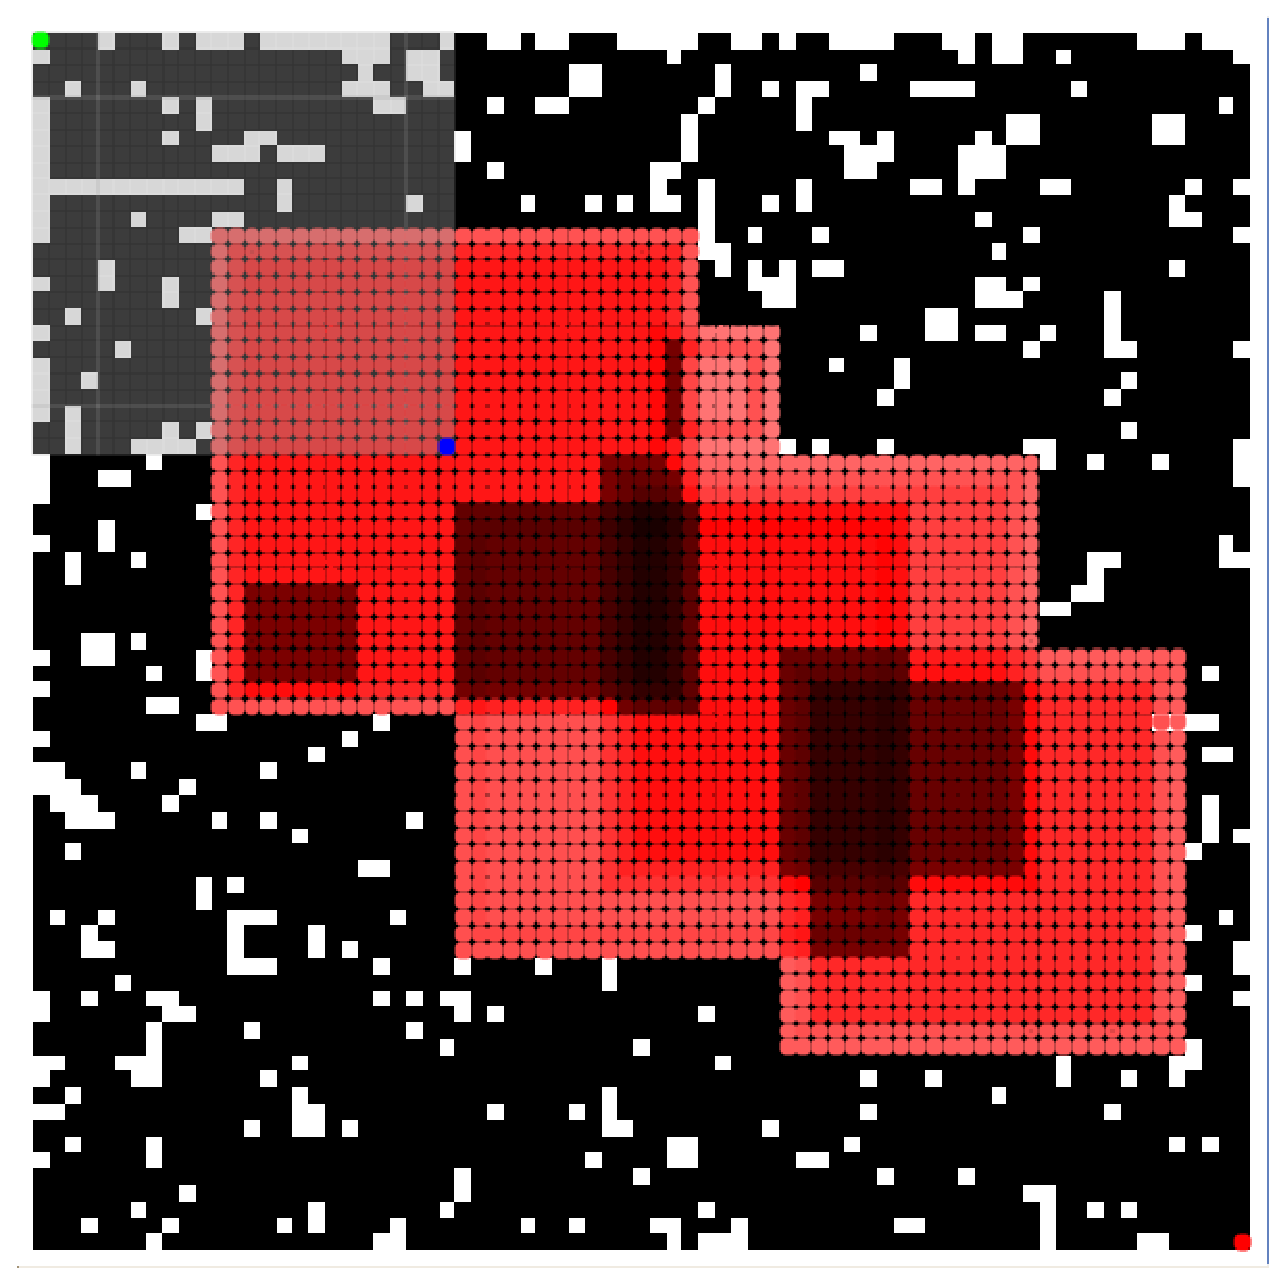
\includegraphics[width=3.5in]{modstarlite/75x75envPropertiesExample}
%\caption{A 75 x 75 Visualized Grid Environment}
%\label{fig:75x75envExample}
%\end{figure}
%
%A simple representation of 2-D grid environment is given in Figure \ref{fig:75x75envExample}. In this figure, white cells are obstacles and black cells are moveable ones. Agent can traverse all cells except for white ones. The UAV agent is initially placed on upper leftmost cell and painted as green. The target locates at the bottom rightmost cell and marked as dark red color. The lighter-red square areas represent threat zones. As two threat zones overlaps, the overlapped area becomes darker to represent that risk is increased exponentially on this area. The fogged gray area around UAV agent represents agent's vision range. As agent moves, this area is dragged. Thus, agent always chooses the best available cell within her vision range with respect to actual target. This temporary target is marked with blue.

\subsection{The Components and Variables}
MOD* Lite is the multi-objective extension of D* Lite. It can be applied to any multi-objective search problem where costs can change by time. Considering formal definition; $S$ denotes the set of states in search problem. $s_{start} \in S$ and $s_{goal} \in S$ are the initial and final (target) states, respectively. $pred(s) \subseteq S$ and $succ(s) \subseteq S$ can be used to find predecessors and successors of given state, $s$. The heuristic function $h(s, s')$ which estimates costs between $s$ and $s'$, cost function $c(s, s')$ which represents the actual cost traversing from $s$ to $s'$, actual cost function $g(s)$ and the $rhs(s)$, one-step-lookahead values of $g(s)$ functions are all inherited from D* Lite. However, as we have to consider more than one objective, these functions are to return vector values of scalars instead of scalars. Thus, $rhs(s)$ satisfies the condition

\[ rhs(s) = \left\{ \begin{array}{lc}
ObjectiveVector.MIN & \mbox{if $s=s_{start}$}\\
nonDom_{s' \in pred(s)}(sum(g(s'), c(s', s))) & \mbox{otherwise}.\end{array} \right. \] 

where ObjectiveVector.MIN stands for a base vector with $n$ values corresponding to $n$ objectives. Any value  could be $0$ or $\infty$ whether the relevant objective is to be minimized or maximized, respectively. $sum()$ function implements vector summation and $nonDom()$ function returns the set of best non-dominated vectors corresponding to predecessors of any state $s$. Note that $nonDom()$ constructs a list of objective vectors, $rhs(s)$ and $g(s)$ function values are represented as a \textit{lists of objective vectors} where each objective vector in this list is non-dominated with others. An objective vector is a structure that holds values for each objective defined by problem (minimization or maximization). In case of having more than one objective, it is possible that there are more than one paths to a particular state that do not dominate each other. That's why each state might be represented by several vectors. In case we need to compare if one state is better than another, two sets of their vectors need to be compared as formulated below.

\begin{definition}
It can be said that $u=[u_1,\cdots,u_n]$ \textit{completely dominates} $v=[v_i,\cdots,v_n]$ iff $\forall i \; u_i \le v_i$ and $\exists j \;\; u_j < v_j$ where $1 \le i, j \le n$.
\end{definition}

Assume that $\upsilon_{1}=\{[2,5],[3,4]\}, \upsilon_{2}=\{[6,1],[5,2]\}, \upsilon_{3}=\{[3,5]\}$ are lists of objective vectors for three states. $\upsilon_{1}$ and $\upsilon_{2}$ are non-dominated whereas $\upsilon_{1}$ completely dominates $\upsilon_{3}$. 

Note that "greater than", "smaller than" and "equals" for scalar value comparison are replaced by "completely dominates", "completely dominated by" and "multi-objectively equals" for vectors of scalars. Non-domination is introduced and handled as the fourth case.

D* Lite introduces local consistency and inconsistency concepts with respect to comparing $g(s)$ and $rhs(s)$. A state is called {\it locally consistent} when $g(s)$ and $rhs(s)$ are equal, and {\it locally inconsistent} otherwise. A locally inconsistent state is referred to as locally underconsistent if $g(s)<rhs(s)$ or locally overconsistent if $g(s)>rhs(s)$. In case of non-domination of these functions, we introduce the concept of {\it local non-consistency}.

\begin{definition}
A state is referred as \textit{locally non-consistent} if its $g(s)$ and $rhs(s)$ values are non-dominated to each other. This inconsistency condition causes the state to reside on more than one solution because it can be understood that two or more predecessors of $s$ are non-dominated to each other.
\end{definition}

Other multi-objective operations are introduced in following subsections. The overall flow of MOD* Lite with PLAN() as main procedure is given in Algorithm \ref{algMain}.

%% The main algorithm.
\begin{algorithm}
	\caption{Main loop of MOD* Lite}
	\label{algMain}
	%\begin{spacing}{0.5}
	{\fontsize{9}{9}\selectfont
    \begin{algorithmic}[1] % line numbering every line
      \Function{plan()}{}
      	\State initialize()
      	\State computeMOPaths()
      	\While{$true$}
    	      	\State solutionPaths = generateMOPaths()
    	      	\If{solutionPaths = null} there is no known path \EndIf
    	      	\State Wait for any weight cost to change;
    	      	\If{Any weight cost changes}
    	      		\State $k_{m}$ = sum($k_{m}$, h($s_{goal}$, $s_{start}$))
    	      		\ForAll {Changed weight costs of edges(u,v)}
    	      			\State Update cost c(u,v)
    	      			\State updateVertex(u)
    	      		\EndFor
		      	\State computeMOPaths()
    	      	\EndIf
		\EndWhile
  	  \EndFunction
      \Statex      
      \Function{calculateKey}{s}
      	\State $k_{2}$(s)= nonDom(g(s), rhs(s))
      	\State $k_{1}$(s) = sum(h($s_{start}$, s), $k_{m}$, $k_{2}$(s))
      	\State \Return $[k_{1}(s), k_{2}(s)]$
      \EndFunction
   	  \Statex
      \Function{initialize()}{}
      	\State $U = \varnothing $
      	\State $k_{m}$ = ObjectiveVector.MIN
      	\ForAll{$s \in S$}
     		\State rhs(s)=g(s)=ObjectiveVector.MAX
     	\EndFor
      	\State rhs($s_{goal}$) = ObjectiveVector.MIN
      	\State U.insert($s_{goal}$, calculateKey($s_{goal}$))
	  \EndFunction
    \end{algorithmic}}
    %\end{spacing}
\end{algorithm}

Basically, D* Lite tries to make all states locally consistent. Locally inconsistent states are maintained in  a priority queue (U) with their key values and expanded considering priority values. However, locally non-consistent states cannot be maintained in such a queue due to the non-domination of their key values, which are also set of objective vectors. If two keys cannot be dominated by each other, they should be criticized in the same manner. Thus, a more convenient structure; a directed acyclic state expansion graph instead of a priority queue which uses topological ordering of states with respect to the key domination, is presented. In this model, the graph (U) contains a set of nodes each represented by a state and its key value. When a state is to be added into U with $insert(state, key)$ operation, key value is compared with all existing nodes' key values. If the new state dominates some state, an edge is introduced from the new state to this state. No edge is introduced in case of equality and non-domination. As a result, incoming and outgoing degrees of a node $s$ correspond to the number of nodes that \textit{dominates} $s$ and the number of nodes that are \textit{dominated by} $s$, respectively. The nodes with incoming degree 0 are the non-dominated nodes where none of other nodes could dominate. $topKey()$ and $topKeys()$ return the key value(s) of nodes with minimum incoming degree. $pop()$ returns and removes the state (all its incident -incoming and outgoing- edges are also removed from the graph) with minimum incoming degree. Another strategy for $pop()$ operation could be removing the state with maximum outgoing degrees where the number of outgoing degree of a state $s$ corresponds to the number of states  dominated by $s$. Also, these two methods could be combined where two topologically ordered lists, one for minimum incoming degrees and the other  for maximum outgoing degrees, are maintained and a state which has both minimum incoming and maximum outgoing degrees according to these lists could be selected. The strategy to be applied can be selected according to application domain requirements. We preferred selecting and removing from minimum incoming degrees list for our application domain. If more than one nodes exist with minimum degree, one of them is selected randomly. $remove(state)$ operation removes a given state and its incident edges from graph. An example of a state expansion graph with states and their corresponding key values is given in Figure \ref{fig:graph1}. Incoming degrees of nodes are given as a list in the figure.

\begin{figure}
\centering
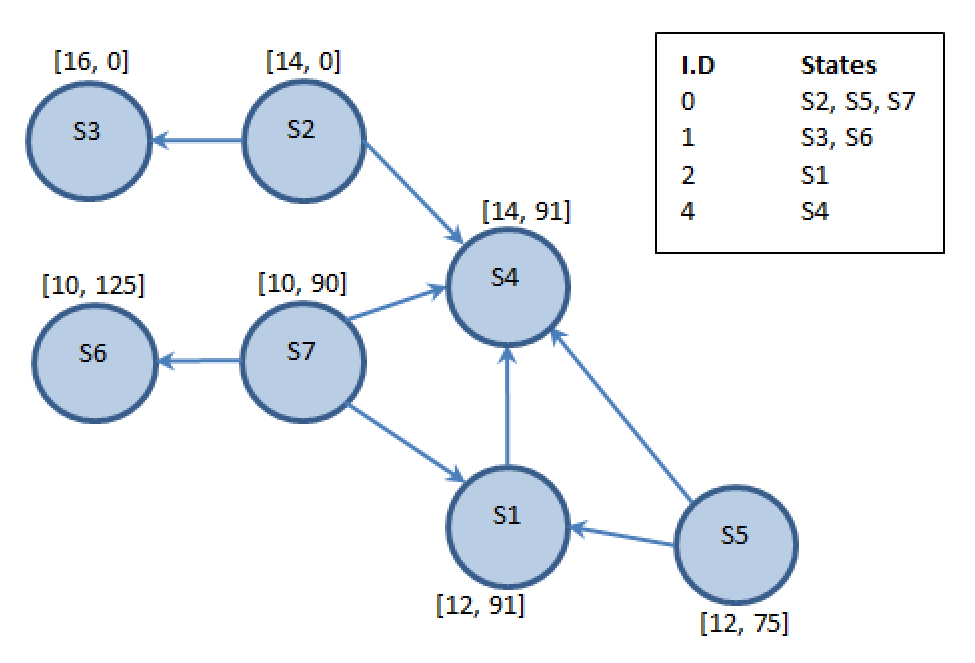
\includegraphics[width=2.0in]{modstarlite/graph1v2}
\caption{Directed Acyclic State Expansion Graph}
\label{fig:graph1}
\end{figure}

Addition of a new state to the state expansion graph is illustrated in Figure \ref{fig:graph2}.  $S8$ is  the new state to be added, the dashed directed edges are established between $S8-S1$, $S8-S4$ and $S8-S5$ because $S8$'s key can only dominate keys of nodes $S1, S4$ and $S5$. None of the existing states' keys can dominate $S8$, so incoming degree of $S8$ becomes 0. This addition also effects the incoming degrees list where the changed positions are highlighted in the figure. Addition of $S8$ increments the incoming degrees of $S1$, $S4$ and $S5$ by 1 so their positions are shifted down.

\begin{figure}
\centering
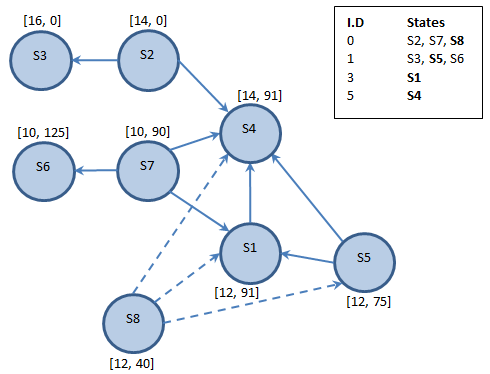
\includegraphics[width=2.0in]{modstarlite/graph2v2}
\caption{State Expansion Graph after Adding State $S8$}
\label{fig:graph2}
\end{figure}

\subsection{Key Formulation}
In the previous subsection, it is stated that the directed acyclic graph structure is used to determine expansion of nodes in state space with their \textit{keys}. The basic idea behind the calculation of keys is similar with D* Lite, with slight modifications. As MOD* Lite is considered in a multi-objective setting, key value is stated as a vector with two components: $k(s) = [k_{1}(s);k_{2}(s)]$ where these components are set of objective vectors. $k_{2}(s)$ is calculated by finding the \textit{non-dominated list} of $g(s)$ and $rhs(s)$, where $k_{2}(s)= nonDom(g(s), rhs(s))$. The other component, $k_{1}(s)$  is calculated as vector summation of $h(s_{start}, s), k_{m}$ and $k_{2}(s)$. Calculation of $k(s)$ can be seen in lines \{2 and 3\} in Algorithm \ref{algMain}. $k_{m}$ is used for heap reordering as defined in  D* Lite.

\begin{algorithm}
	\caption{Update Vertex \& Compute Multi-Objective Paths}
	\label{algUpdate}
    \begin{algorithmic}[1]
   	  \Function{updateVertex}{u}
   	  	\If{$u \neq s_{goal}$}
   	  		\State $rhs(u) = nonDom_{s' \in succ(u)}(sum(c(u,s'), g(s')))$
   	  	\EndIf
   	  	\If{$u \in U$} U.remove(u) \EndIf
   	  	\If{!equals(g(u), rhs(u))}
   	  		\State U.insert(u, calculateKey(u))
   	  	\EndIf
   	  \EndFunction
    	  \Statex
      \Function{computeMOPaths()}{}
		\While{dominatesAll(calculateKey($s_{start}$), U.topKeys())}
		% OR !equals(rhs(s_{start}, g(s_{start}))$}
			\State $k_{old}$ = U.topKey()
	      	\State u = U.pop()
	      	\State $k_{new}$ = calculateKey(u)
	      	\If{$k_{old}$.completelyDominates($k_{new}$) }
	      		\State U.insert(u, $k_{new}$)
	      	\ElsIf{rhs(u).completelyDominates(g(u))}
	      		\State g(u) = rhs(u)
	      		\ForAll{$s \in pred(u)$} $updateVertex(s)$ \EndFor
	      	\ElsIf{g(u).completelyDominates(rhs(u))}
	      		\State g(u) = ObjectiveVector.MAX
	      		\ForAll{$s \in pred(u) \cup \{u\}$} $updateVertex(s)$ \EndFor
	      	\Else
	      		\State g(u) = nonDom(g(u), rhs(u))
	      		\ForAll{$s \in pred(u)$} $updateVertex(s)$ \EndFor
	      	\EndIf
		\EndWhile
	  \EndFunction
	\end{algorithmic}
\end{algorithm}

\subsection{Details of MOD* Lite}
MOD* Lite is based on  D* Lite algorithm as introduced in the previous section. There are fundamental differences due to the structures used and the way the solution paths are maintained. The pseudocode of MOD* Lite is given in Algorithms \ref{algMain}, \ref{algUpdate} and \ref{algPathGen}.

First of all, searching order of MOD* Lite is from goal to start state, like D* Lite. The main function of MOD* Lite first calls $initialize()$ to set up the execution in Algorithm \ref{algMain}. This function calculates the key value for goal state, adds it into U and sets the rhs value to a \textit{MIN} objective vector, which has minimized n values for n-objectives. These values can be $0$ for minimized-objective and $\infty$ for maximized-objective. Then, proper $g(s)$ values are calculated considering all objectives with $computeMOPaths()$. Finally, paths are generated with these $g(s)$ values. If a weight cost is changed in the environment, corresponding states are re-expanded and only related weights are updated. Notice that this cost change might happen for only one objective or several objectives at the same time.

The $computeMOPaths()$ pseudocode is given in Algorithm \ref{algUpdate} line \{7\}. The termination criteria of this function is where the key of $s_{start}$ dominates all the top keys returned from U. Until it terminates, the top state is sequentially selected from top states of U and expanded. While expanding a state, the domination between g and rhs values of corresponding state is observed. If $rhs(s)$ values completely dominate $g(s)$ values, local underconsistency case occurs. We apply the same strategy with D* Lite, update g value with rhs and update weights for all predecessors of s with $updateVertex()$. If $g(s)$ values completely dominate $rhs(s)$ values, the case is locally overconsistency. Simply g value for this state is set as \textit{MAX} objective vector, which is $\infty$ for minimized-objective and $0$ for maximized one, and current state weight is updated with its predecessors' weight. The third case occurs when g and rhs values can not completely dominate each other, \textit{locally non-consistency}. In this case, g value is updated with non-dominated values of g and rhs values and again predecessors of current state is updated. Keeping non-dominated values of g and rhs enables to keep track of each non-dominated successors' information.

To update a weight of a state, MOD* Lite uses $updateVertex(u)$ shown in Algorithm \ref{algUpdate} line \{1-6\}. It simply adds corresponding state to or removes from U according to given criteria. While updating $rhs(u)$ except goal state, non-dominated objective values of multi-objectively summed $c(u,s')$ and $g(s')$ are established and used.

After state expansion operation is finalized and corresponding $g(s)$ values are set, multi-objective paths are generated via these $g(s)$ values by given pseudocode in Algorithm \ref{algPathGen}. Path generation is achieved in two phases: setting parent(s) for each non-dominated successor of expanding state and constructing paths by following (backtracking) these parents. The first phase is performed from the start to the goal state whereas the second is from the goal to the start state. 

A queue is used to keep track of expanding states which is shown in line \{2\}. This queue initially has $s_{start}$ only. Thus, starting from $s_{start}$, the while loop iterates until this queue becomes empty. Finding a goal state is not considered as a termination criteria because other non-dominant paths might be available. As expanding a state, we refer to set \textit{it} as a parent to its successors indicated between lines \{7-36\}.

Before expansion of a state $s$, non-dominated successors are found first with respect to multi-objective summation of $c(s,s')$ and $g(s')$ as shown in line \{5\}. If a successor $s'$ is found in non-dominated successors list, it has a potential to have $s$ as a parent. For each non-dominated successor $s'$, first parents list of $s$ is checked. If $s$ does not have any parent, which only occurs iff $s=s_{start}$, for sure $s'$ does not have any parent as well. In this case, $s$ is added  as a parent of $s'$ with corresponding cost $c(s,s')$. Parents of a state are kept in a map where keys of this map are parents and values are cumulative costs which is consumed to reach that state from start through corresponding parent. These costs are used to determine elimination of existing parents when a new one is considered to be added. This idea will be elaborated later.

% Indentations are used make visualization better.
\begin{algorithm}
	\caption{Path Generator Algorithm}
	\label{algPathGen}
    \begin{algorithmic}[1]
    		\Function{generateMOPaths()}{}
			\State expandingStates.add($s_{start}$)
    			\While{!expandingStates.isEmpty()}
    				\State s = expandingStates.poll()
				\State nonDomSuccs = $nonDom_{s' \in succ(s)}$(sum(c(s, s'), g(s'))
    				\ForAll{$s'\in nonDomSuccs$}
    					\If{s.parents() = null}
    						\State s'.parents().put(s, c(s, s'))
    					\Else
    						\State cumulativeC = sum(c(s, s'), s.parents().values())
    						\If{s'.parents() = null}
    							\State s'.parents().put(s, cumulativeC)
    						\Else
							\ForAll {$s'' \in s'.parents()$}
								\If{equals(s'.parents(s''), cumulativeC) OR completelyDominates( s'.parents(s''), cumulativeC)}
									\State \textbf{break}
								\ElsIf{completelyDominates(cumulativeC, s'.parents(s''))}
									\State s'.parents().remove(s'')
									\State s'.parents().put(s, cumulativeC)
								\Else
									\ForAll{$cC \in cumulativeC$}
										\ForAll{$eC \in s'.parents(s'')$}
											\If{eC.equals(cC) OR eC.dominates(cC)}
												\State cumulativeC.remove(cC) 
												\State \textbf{break}
											\ElsIf{cC.dominates(eC)}
												\State s'.parents(s'').remove(eC) 
												\State \textbf{break}
											\EndIf
										\EndFor
										\If{s'.parents(s'') = null}
											\State s'.parents().remove(s'')
										\EndIf
									\EndFor
									\If{!cumulativeC = null}
											\State s'.parents().put(s, cumulativeC)
									\EndIf
								\EndIf
							\EndFor    						
    						\EndIf
    					\EndIf
    					\If {s'.parents.contains(s) AND !expandingStates.contains(s')}
    						\State expandingStates.add(s')
    					\EndIf
    				\EndFor
    			\EndWhile
    			\State solutionPaths = construct paths recursively traversing parents
    			\State \Return solutionPaths
    		\EndFunction
	\end{algorithmic}
\end{algorithm}

If $s$ has predefined parents (starting from \{9\}), a cumulative total cost is calculated for $s'$ in line \{10\}. This cost is multi-objective summation of $c(s, s')$ and aggregated cost values of parents of $s$. Notice that the algorithm proves that parents' costs of a state are always non-dominated to each other, so the aggregated cost values contain \textit{all} parents' \textit{all} costs. These cost values express all non-dominated solution costs to reach that state. If $s'$ does not have any parent up to now (\{11\}), $s$ is added as a parent of $s'$ with cumulative cost. Else, each existing parent of $s'$, say $s''$ should be compared with the cumulative cost. These operations are shown in lines between \{13-32\}. Here, if $s''$ has same cost with or better cost (determined by completely domination term) than cumulative cost, needless to say that $s$ is not required to be added as a parent to $s'$. Otherwise, if cumulative cost completely dominates $s''$, it can be inferred that one can reach $s'$ from $s$ in a better way than $s''$. Thus, $s''$ is removed from parents of $s'$ and $s$ is added with the cumulative cost. The fourth possibility occurs when costs of $s''$ and cumulative costs do not completely dominate each other. In this situation, each cost in cumulative costs is compared with each cost of $s''$ costs. Equality or domination probabilities causes to remove corresponding cost from its list. At the end of the comparison, $s''$ is removed from parents of $s'$ if all of its costs are dominated (lines \{29-30\}) and $s$ is added as a parent if cumulative costs still have non-dominated cost (lines \{31-32\}).

After organizing parents of $s'$, it is decided to expand it in following iterations. If $s$ is successfully added as a parent and expanding states queue does not already have it, $s'$ is added to the tail of the queue. This can be seen in lines \{33-34\}.

When all non-dominated parents are properly set from start to goal state, these parents can be followed recursively starting from goal towards start state and multi-objective paths are constructed. Finally, all found paths have non-dominated path costs regarding to each other.

\section{A Multi-Objective Genetic Path Planner : MOGPP}

Many real-life optimization problems are NP-hard where optimal solutions could not be found in polynomial time. As evolutionary computing methods are classified as stochastic soft-computing methods and can be applied to NP-hard problems, many genetic algorithms are developed with respect to this problem \cite{Pangilinan}, \cite{Peng_Xu_Zhang:2011}. In order to show efficiency and effectiveness of MOD* Lite algorithm in terms of time and solution quality, we developed a stochastic evolutionary algorithms (a multi objective genetic path planner named MOGPP)  as an alternative soft computing genetic realization for finding paths considering multiple objectives and conducted a comparative experimental study. MOGPP is designed as a complete algorithm, which could eventually find non-dominated valid path(s) from initial location to target one, if any exists. It does not guarantee to find optimal solutions and hence Pareto front in that respect.

In MOGPP, a chromosome encodes a valid path from an initial location to a target one specifying a legal solution for the problem. Each gene in a chromosome is a \textit{cell} in this valid path. Chromosomes are of varying lengths as solution paths are not fixed. The fitness function used in MOGPP is given as follows; \[F(i) = [\dfrac{1}{L(i)^{2}}, \dfrac{1}{R(i)^{2}}] \] where $F(i)$ is the fitness of chromosome $i$, $L(i)$ is the length of the path and $R(i)$ is the exposed risk of this path.  Our fitness calculation favors paths that are shorter and safer. 

We used roulette-wheel selection mechanism to determine parents for mating chromosomes through crossover  operation. As a single chromosome stands for a valid path in MOGPP, newly generated children should also obey this rule. Thus, genetic operations must guarantee that newly generated children are consistent and exhibit valid paths. For crossover operation used in MOGPP, assume that two parents' paths are represented by 
\begin{gather*}
P(i)=\lbrace \varsigma, ..., c_{i-1}, c_{i}, c_{i+1}, ..., \tau \rbrace \\
P(j)=\lbrace \varsigma, ..., c_{j-1}, c_{j}, c_{j+1}, ..., \tau \rbrace
\end{gather*}
for $i$ and $j$ individuals. $\varsigma$ and $\tau$ shows initial and target locations, respectively. While crossover, an intersected cell of these paths is determined. Then, each path is split up into two sub-paths referencing by this cell. If this cell is $c_{i} = c_{j}$, the splitting operation is done as follows
\begin{gather*}
P(i)_{1}=\lbrace \varsigma, ..., c_{i-1} \rbrace, 
P(i)_{2}=\lbrace c_{i}, c_{i+1}, ..., \tau \rbrace \\
P(j)_{1}=\lbrace \varsigma, ..., c_{j-1} \rbrace, 
P(j)_{2}=\lbrace c_{j}, c_{j+1}, ..., \tau \rbrace
\end{gather*}
The concatenation of swapped sub-paths generate new individuals
\begin{gather*}
P'(i)=\lbrace P(i)_{1}, P(j)_{2} \rbrace, 
P'(j)=\lbrace P(j)_{1}, P(i)_{2} \rbrace 
\end{gather*}
$P'(i)$ and $P'(j)$ are the new paths for parents $i$ and $j$.
%Also, a visualization  of crossover operation is given in Figure \ref{fig:xover}.

%\begin{figure}
%\centering
%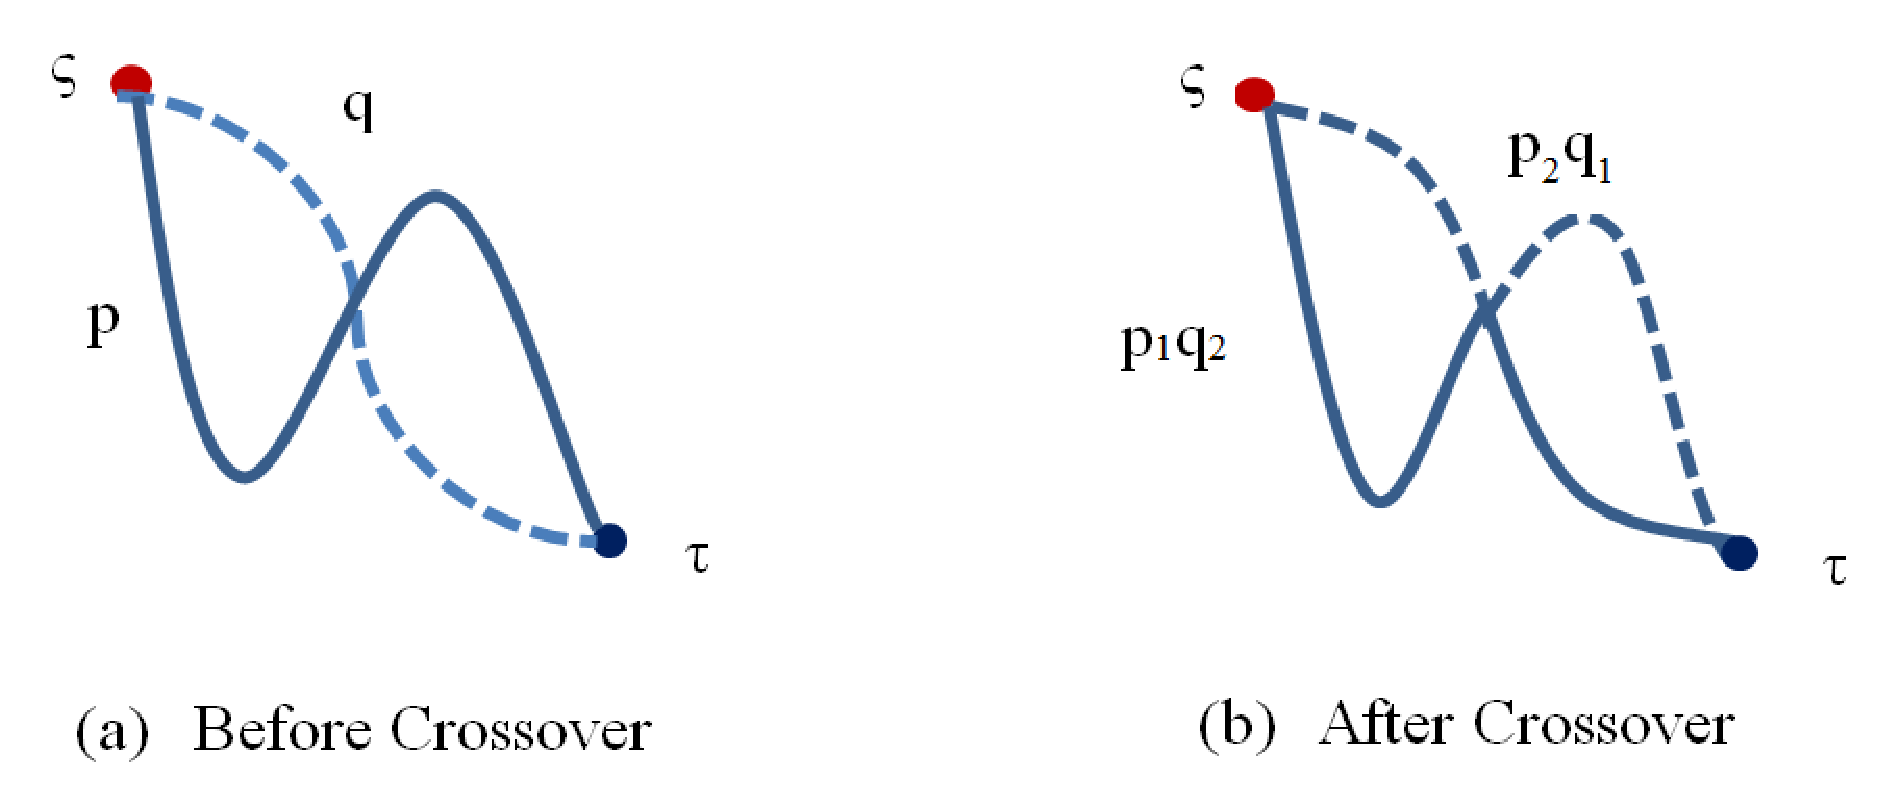
\includegraphics[width=2.5in]{mogpp/xover}
%\caption{Crossover Operation}
%\label{fig:xover}
%\end{figure}

Concerning mutation,  a cell from individual's path is selected randomly first. This cell is the reference point to split up the path into two sub-paths. Then, the sub-path which contains target location is thrown away and a random path to the target is generated instead. %The visualization of mutation is given in Figure \ref{fig:mutation}.

%\begin{figure}
%\centering
%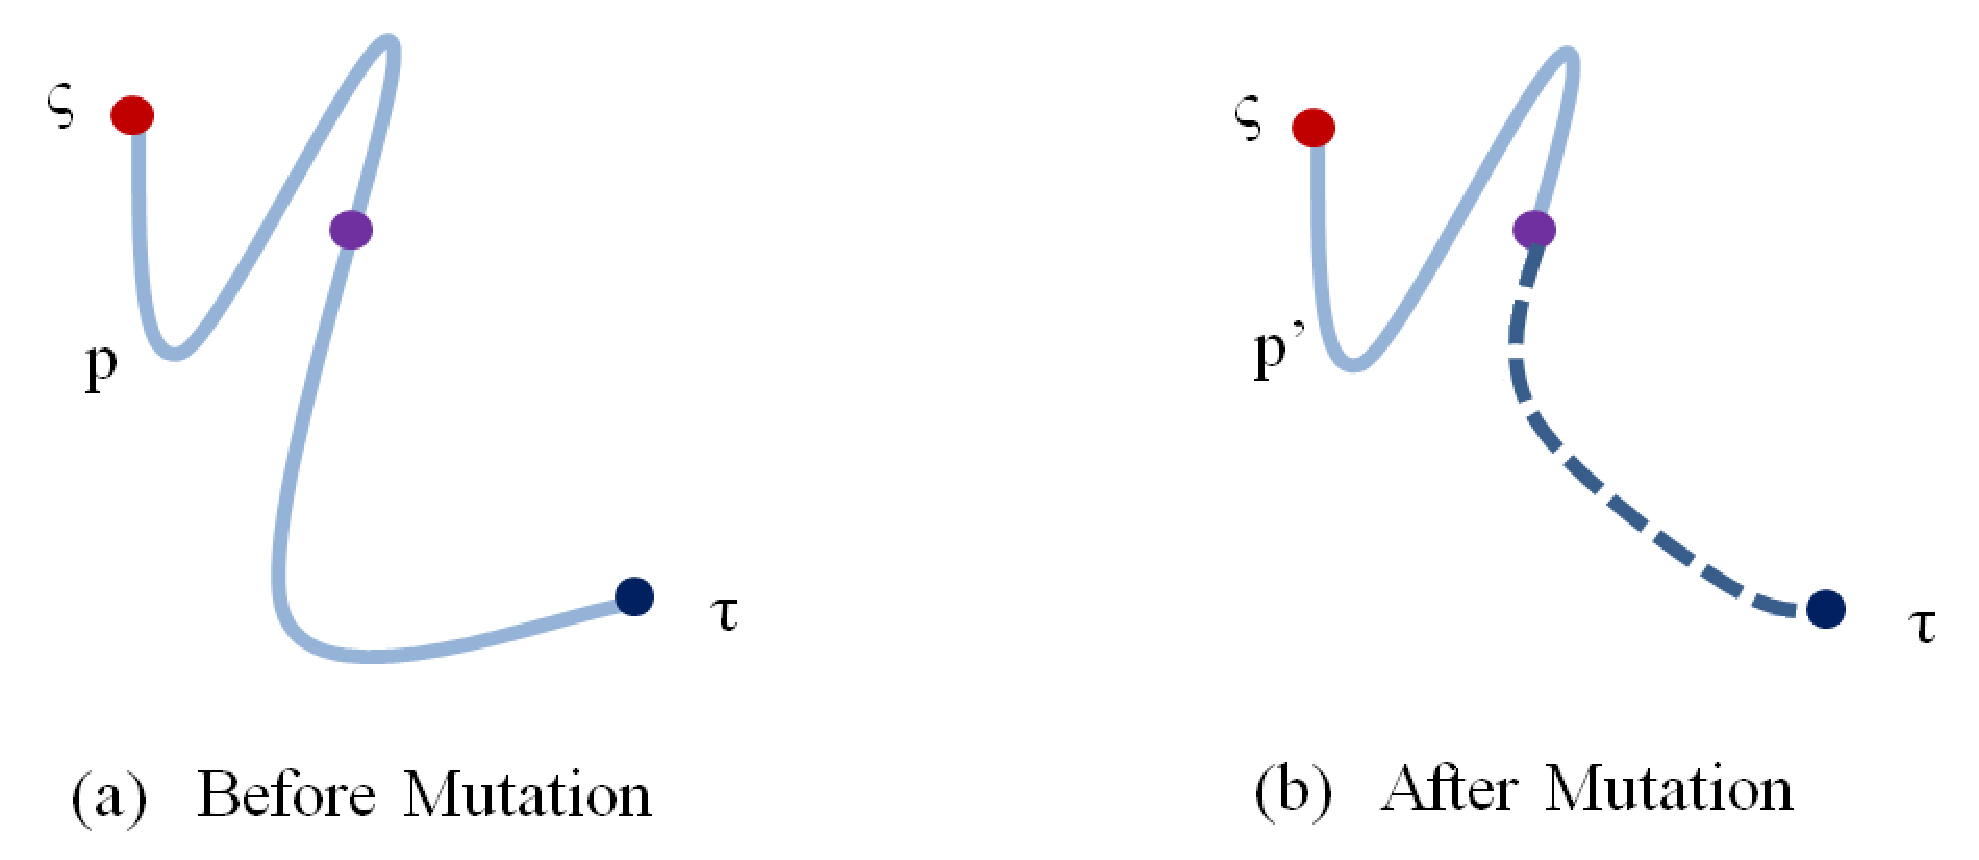
\includegraphics[width=2.5in]{mogpp/newMutation}
%\caption{Mutation Operation}
%\label{fig:mutation}
%\end{figure}


%As mentioned above, MOGPP is designed based on a simple classic genetic algorithm structure. Main loop of MOGPP is given in Algorithm \ref{algMOGPP}.

%\begin{algorithm}
%	\caption{MOGPP : Main Loop}
%	\label{algMOGPP}
%    \begin{algorithmic}[1]
%    	  \Function{evolve()}{P}
%	  	\State $P' = \varnothing$
%	  	\State $P'.addAll(elites(P))$
%	  	\While{$P'.size < P.size$}
%	  		\State $parents = selectParents(P)$
%	  		\State $crossover(parents)$
%	  		\State $mutate(parents)$
%		  	\State $P'.addAll(parents)$
%	  	\EndWhile
%	  	\State \Return $P'$
%      \EndFunction
%   	  \Statex
%      \Function{initializePopulation()}{}
%      	\State $P = \varnothing$
%      	\For{$i = 1 \to POPULATION\_SIZE$}
%      		\State $P(i) = generateRandomPath(\varsigma, \tau)$
%      	\EndFor
%      	\State $evaluate(P)$
%		\State \Return $P$
%	  \EndFunction
%	  \Statex
%	  \Function{plan()}{}
%      	\State $P = initializePopulation()$
%      	\While{$reached\ to\ MAX\_ITERATION$}
%    	      	\State $P = evolve(P)$
%    	      	\State $evaluate(P)$
%		\EndWhile
%		\State \Return $bestIndividuals(P)$
%  	  \EndFunction
%	\end{algorithmic}
%\end{algorithm}

As mentioned above, MOGPP is designed based on a simple classic genetic algorithm structure. At first, random valid paths from initial location ($\varsigma$) to the target ($\tau$) are generated. Notice that these paths do not contain any ties, to simplify and speed up genetic operators' processes.

Each generated path represents an individual in population. These individuals are kept in a directed acyclic graph to cope with multi-objectivity. The vertices and edges represent individuals and domination of multi-objective path costs of these individuals, respectively. If a path cost of an individual dominates to other's, an edge is established between these individuals' vertices. Non domination and equality do not come up with an edge. When an individual is generated and desired to be added to population, the cost function of this individual is compared with existing individuals' costs and required edge connections are established. The directed acyclic graph structure has the same essence and representation with MOD* Lite' s priority structure, which was detailed in previous section.

After population initialization, all individuals are evaluated with respect to their fitness functions. The evaluation gives better results when an individual's path is shorter and safer. Total fitness value is calculated by adding all individuals' fitness values multi-objectively. This value increases while population is evolving. The evolution process is applied to all individuals of a population. When a population is evolving, predefined number of best individuals are transferred to new population first. Then, two individuals are selected as parents by roulette wheel selection method. This method gives higher chances to the individuals which have better fitness functions to be selected. After two parents are selected, crossover and mutation is applied with predefined distinct probabilities.

After a predefined number of iterations (the maximum iteration count), algorithm is terminated and elite individuals are taken as multi-objectively best results.  
%Notice that the amount of initially generated individuals - population size -, maximum iteration count of evolution, number of elite individuals selected on each evolution phase, crossover and mutation probabilities should be predefined and set before the execution of MOGPP.

\section{Experimental Results}
\label{chapter:experiments}

The algorithm is tested on various environments with different specifications. MOD* Lite is primarily compared with MOA* that guarantees optimal solutions in fully observable multi-objective problem settings. Our aim is to test the quality of solutions produced by MOD* Lite with respect to optimal ones generated by MOA* ignoring its huge running time costs. Note that MOA* requires exponential time and cannot be used for unknown or partially known environments.  Furthermore, we  compared MOD* Lite with SPEA2 and MOGPP, a classic genetic solution which can be used for finding paths with multi-objective cases.

All algorithms are coded in Java and tested on a Linux environment with hardware Intel(R) Core(TM) i7-2600 CPU @ 3.40GHz and 8 GB of RAM with -Xmx6192m parameter for JVM.

All tests are done on 2-D grid maps as detailed in Subsection \ref{envProperties}. In these tests, the agent tries to find available non-dominated best paths with respect to two objectives, path length and risk taken from threat zones. Thus, the agent endeavors to minimize both objectives and tries to find \textit{shortest} and \textit{safest} paths.

For all test cases, several parameters of MOGPP algorithm must be tuned. For instance; the number of elite individuals is taken as $5$, population count and maximum number of iterations are $50$, and cross-over and mutation ratios are taken as $0.8$ and $0.05$, respectively. As MOGPP constructs initial paths randomly, each execution of the algorithm might not give exactly the same results at the same execution time even the maps are equal. Thus, all given execution times and selected paths are considered as the average of 10 different runs of MOGPP. Similar parameter tuning must be done for SPEA2 as well. For the sake of equitable testing environment, we keep all parameters same with MOGPP. We also set archive count as $50$. 

\subsection{Fully Observable Tests}

First of all, it must be shown that MOD* Lite is complete and gives optimal and/or acceptably sub-optimal results in fully observable environments. The performance comparison is done in two dimensions, execution times and paths they generate (path quality), respectively.

In the first set of tests, randomly generated fully observable maps with different sizes $m \times m$ (20 x 20, 40 x 40, 60 x 60, 80 x 80, 100 x 100, 120 x 120, 140 x 140 and 160 x 160) are used. Each of these maps have nearly 25\%-30\%  threat zones and 14\%-16\%  obstacles. Agent's initial and target locations are taken as $(1, 1)$ and $(m, m)$, respectively. For this case, execution times and generated paths' costs for different sized maps are given in Figure \ref{fig:rand_fully} and Table \ref{table:randPaths}. Note that in Table \ref{table:randPaths}, solutions reported by the algorithms are given as non-dominated pairs of two numbers, the first one is the length of the path, the second one is the accumulated risk value through that path, both of which to be minimized. Concerning solution quality, MOA* finds optimal results and MOD* Lite finds optimal or acceptably sub-optimal results while its running times are better than those of MOA*. Although MOGPP works on similar times with MOD* Lite, it fails to find optimal or sub-optimal paths especially for large scaled maps. Also it is important to emphasize that MOGPP does not guarantee Pareto optimum and that's why the results are not optimal or sub-optimal. We could set maximum iteration and population count to larger numbers to have converge on path quality, but this would increases execution times exponentially. Thus, more modest parameters are chosen for MOGPP to enforce the algorithm to yield reasonable results within expected time. In this test, we can also see that SPEA2 yields results with better execution time with respect to other algorithms, however path qualities are not satisfactory. All the results are dominated by both MOD* Lite and MOA* results, and only several of them are non-dominated with MOGPP results. Changing the parameters of SPEA2 will eventually give better path qualities, but again execution time will increase exponentially.
 
Notice that taken risk values depend on environmental properties and should not be compared between different sized maps.

\begin{figure}
\centering
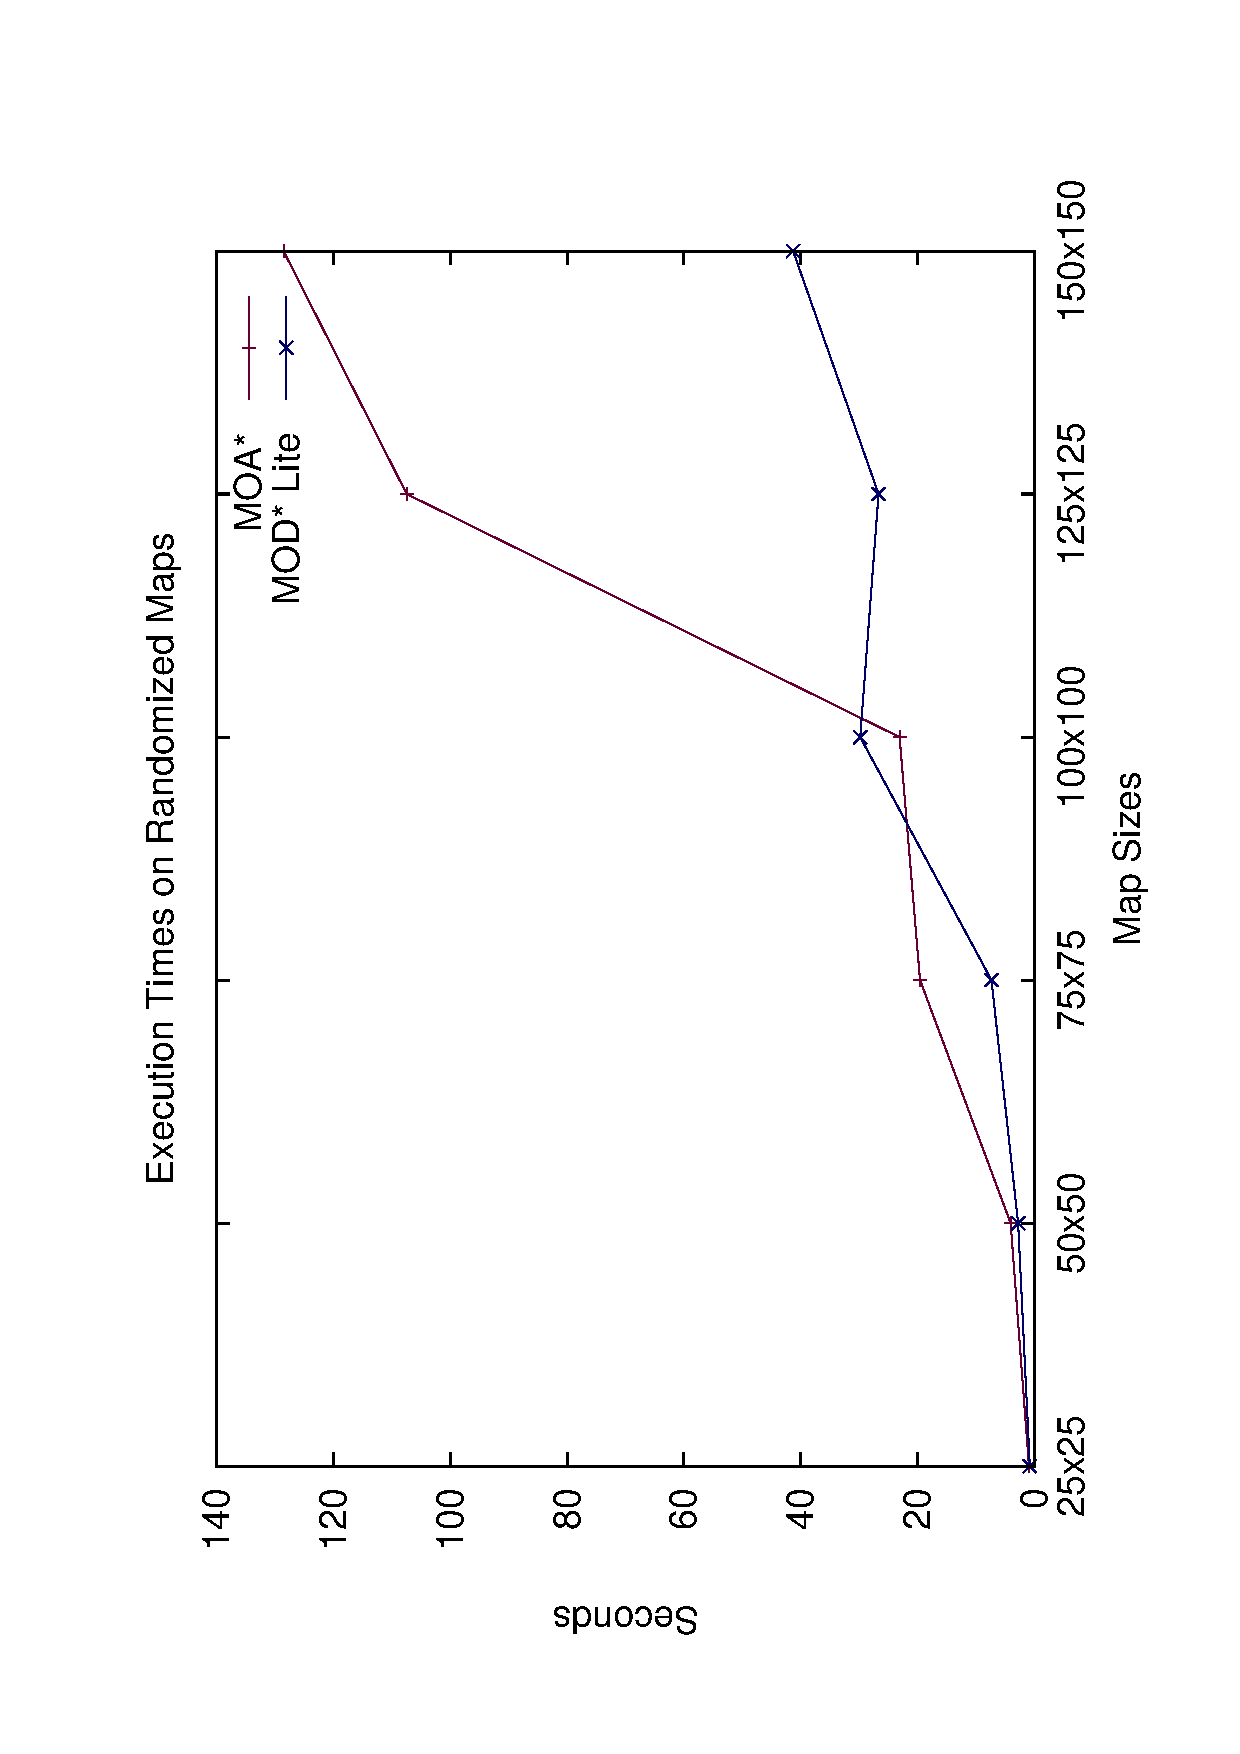
\includegraphics[scale=0.45]{experimental/randomized}
\caption{Execution Times of Randomly Generated Fully Observable Maps}
\label{fig:rand_fully}
\end{figure}

\begin{table}[ht]
	\caption{Non-dominated Path Costs For Randomized Maps}
	\centering
    \begin{tabular}{l l l l l}
        \hline
        Map Size	&  MOD* Lite	&	MOA*		&	MOGPP		&	SPEA2 \\ [0.5ex] \hline
        20 x 20		&	(39,90)		&	(39,90)		&	(41,916)	&	(40,1028)
		   \cr		&	(43,0)		&	(43,0)		&	(43,408)	&	(52,916)
		   \cr		&				&				&				&	(54, 784)
   		   \cr		&				&				&				&	(56, 662)
		   \cr		&				&				&				&	(60, 395)\\
		   \\ 
        40 x 40		&	(79,9)		&	(79,9)		&	(89,2789)	&	(101, 1839)
		   \cr		&	(81,0)		&	(81,0)		&	(103,1239)	&	(103, 1647)
		   \cr		&				&				&	(105,296)	&	(107, 1412)
		   \cr		&				&				&	(105,296)	&	(117, 1153)
   		   \cr		&				&				&	(105,296)	&	(119, 1011)\\
		   \\
		60 x 60		& 	(119,0)		&	(119,0)		&	(151,1970)	&	(158,2016)
		   \cr		&				&				&	(169,549)	&	(176, 1002)
		   \cr		&			  	&				&	(181,426)	&	\\
		   \\
        80 x 80		& 	(159,198)	&	(159,58)	&	(213,6382)	&	(242, 8567)
		   \cr		& 	(161,0)		&	(161,0)		&	(237,2007)	&	(248,2741)
		   \cr		& 				&				& 	(263,1581)	&	(286,1492)
		   \cr		& 				&				& 	(269,955)	&	
		   \cr		& 				&				& 	(285,942)	&	\\
		   \\
        100 x 100	&	(199,885)	&	(199,885)	&	(285,15804)	&	(282,21363)
		   \cr    	&	(201,708)	&	(201,708)	&	(295,14130)	&	(298, 14600)
		   \cr    	&	(203,0)		&	(203,0)		&	(299,14099)	&	(302, 4348)
		   \cr	  	& 				&				&	(305,10979)	&	
		   \cr	  	& 				&				&	(341,9851)	&	
		   \cr	  	& 				&				&	(377,177)	&	\\		   
		   \\
        120 x 120	&	(239,0)		&	(238,0)		&	(371,12817)	&	(382, 18313)
		   \cr		&				&				&	(399,7346)	&	(402, 13205)
   		   \cr		&				&				&				&	(420, 12157)
   		   \cr		&				&				&				&	(432, 7562)\\ 		   		   
		   \\
        140 x 140	&	(279,45)	&	(279,45)	&	(445,10920)	&	(448, 11991)
		   \cr		&	(281,42)	&	(285,12)	&	(483,5281)	&	(512, 10109)        
    	   \cr		&				&	(303,0)		&	(515,4000)	&	(530, 9651)
 		   \cr		&				&			 	&	(517,3520)	&	(536, 6981)
   		   \cr		&				&				&				&	(574, 5855)\\ 		   
 		   \\
        160 x 160	&	(319,0)		&	(319,0)		&	(545,7530)	&	(546, 7260)
		   \cr		& 			 	&			 	&	(547,4602)	&	(608, 5427)\\ [1ex]
        \hline
    \end{tabular}
	\label{table:randPaths}
\end{table}

In the second set of tests, each algorithm is executed on handcrafted maps of the same sizes, threat zone and obstacle ratio with randomized tests as indicated in previous test case. These maps are also assumed fully observable and agent's initial and target locations are as farmost cells on diagonal. All handcrafted test environments \textit{guarantee} that at least two non-dominated paths will be available. Execution times are shown in Figure \ref{fig:hand_fully} and generated paths' costs are given in Table \ref{table:handPaths}.

\begin{figure}
\centering
%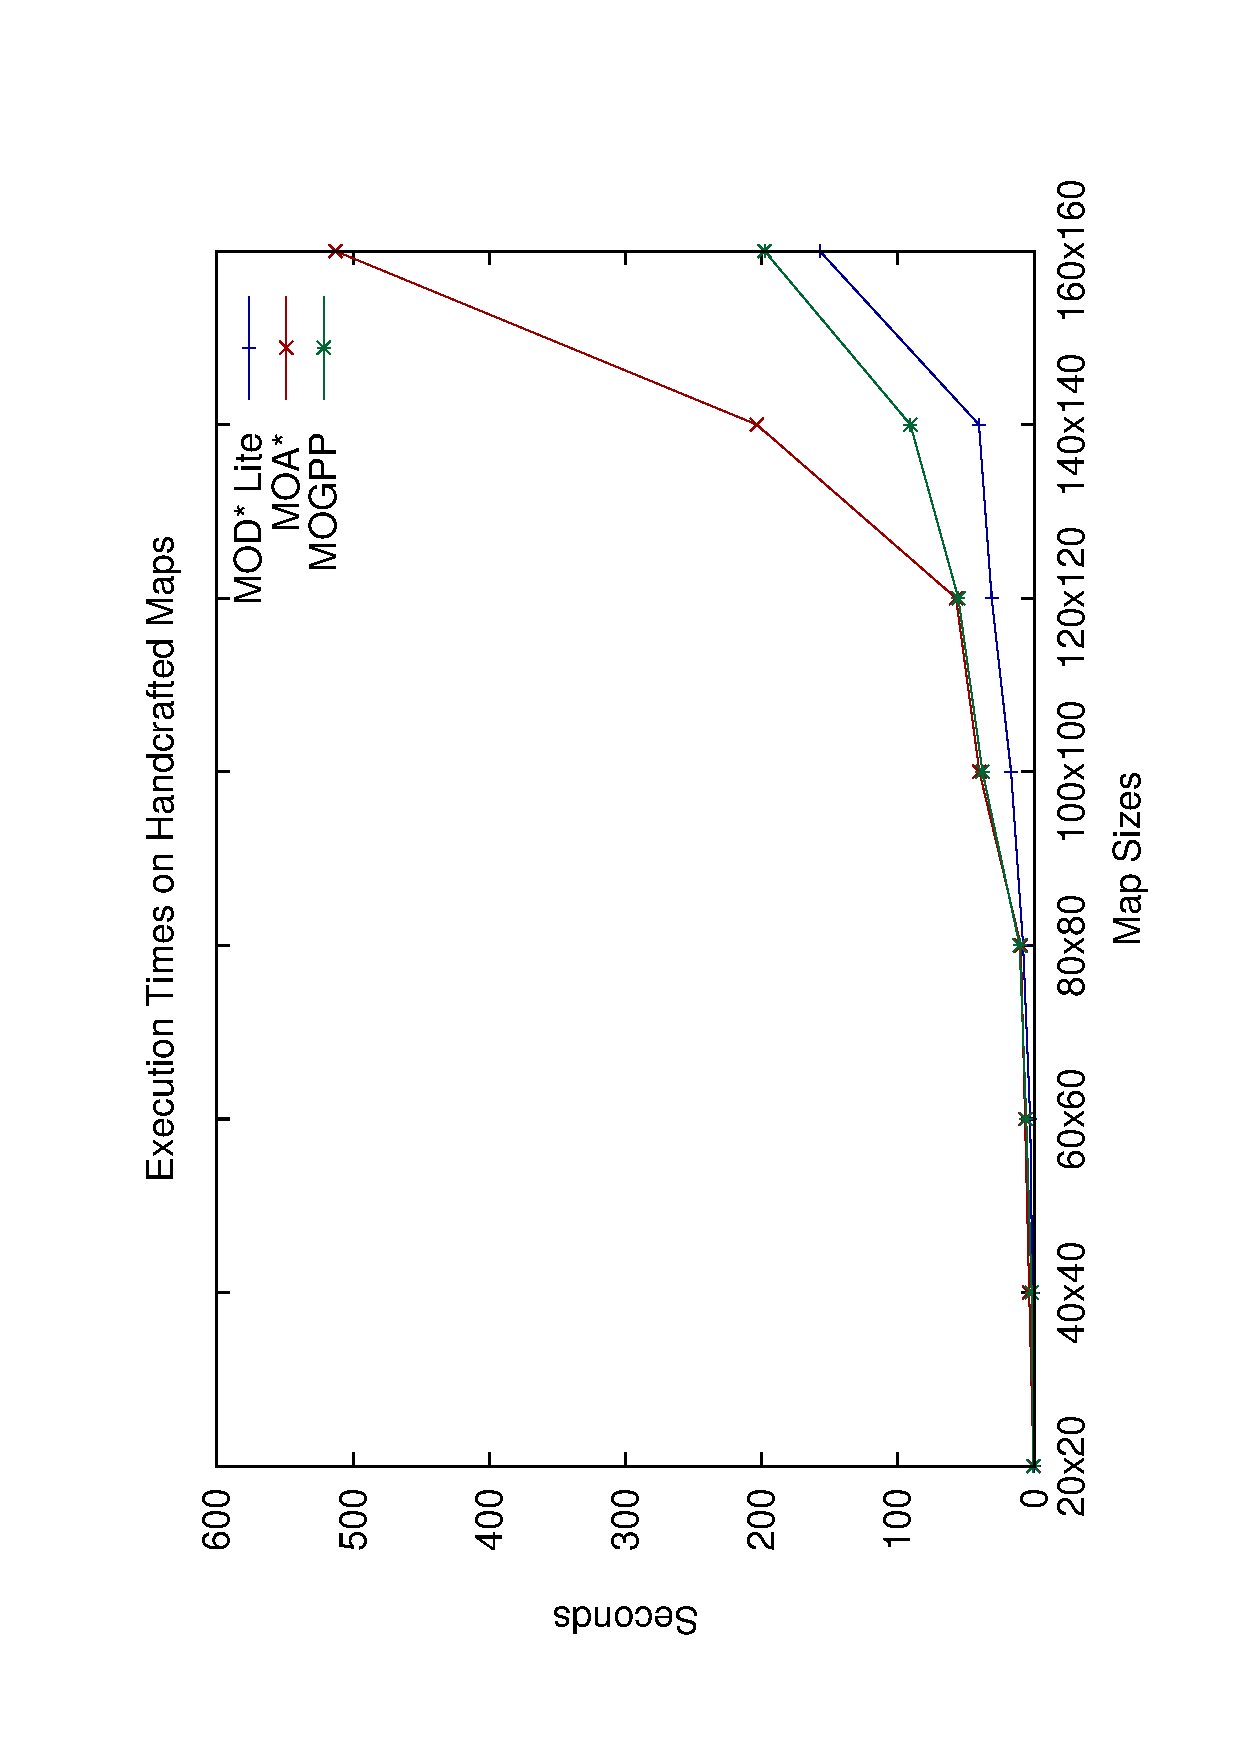
\includegraphics[width=3.7in, height=3in]{experimental/handcrafted_normal}
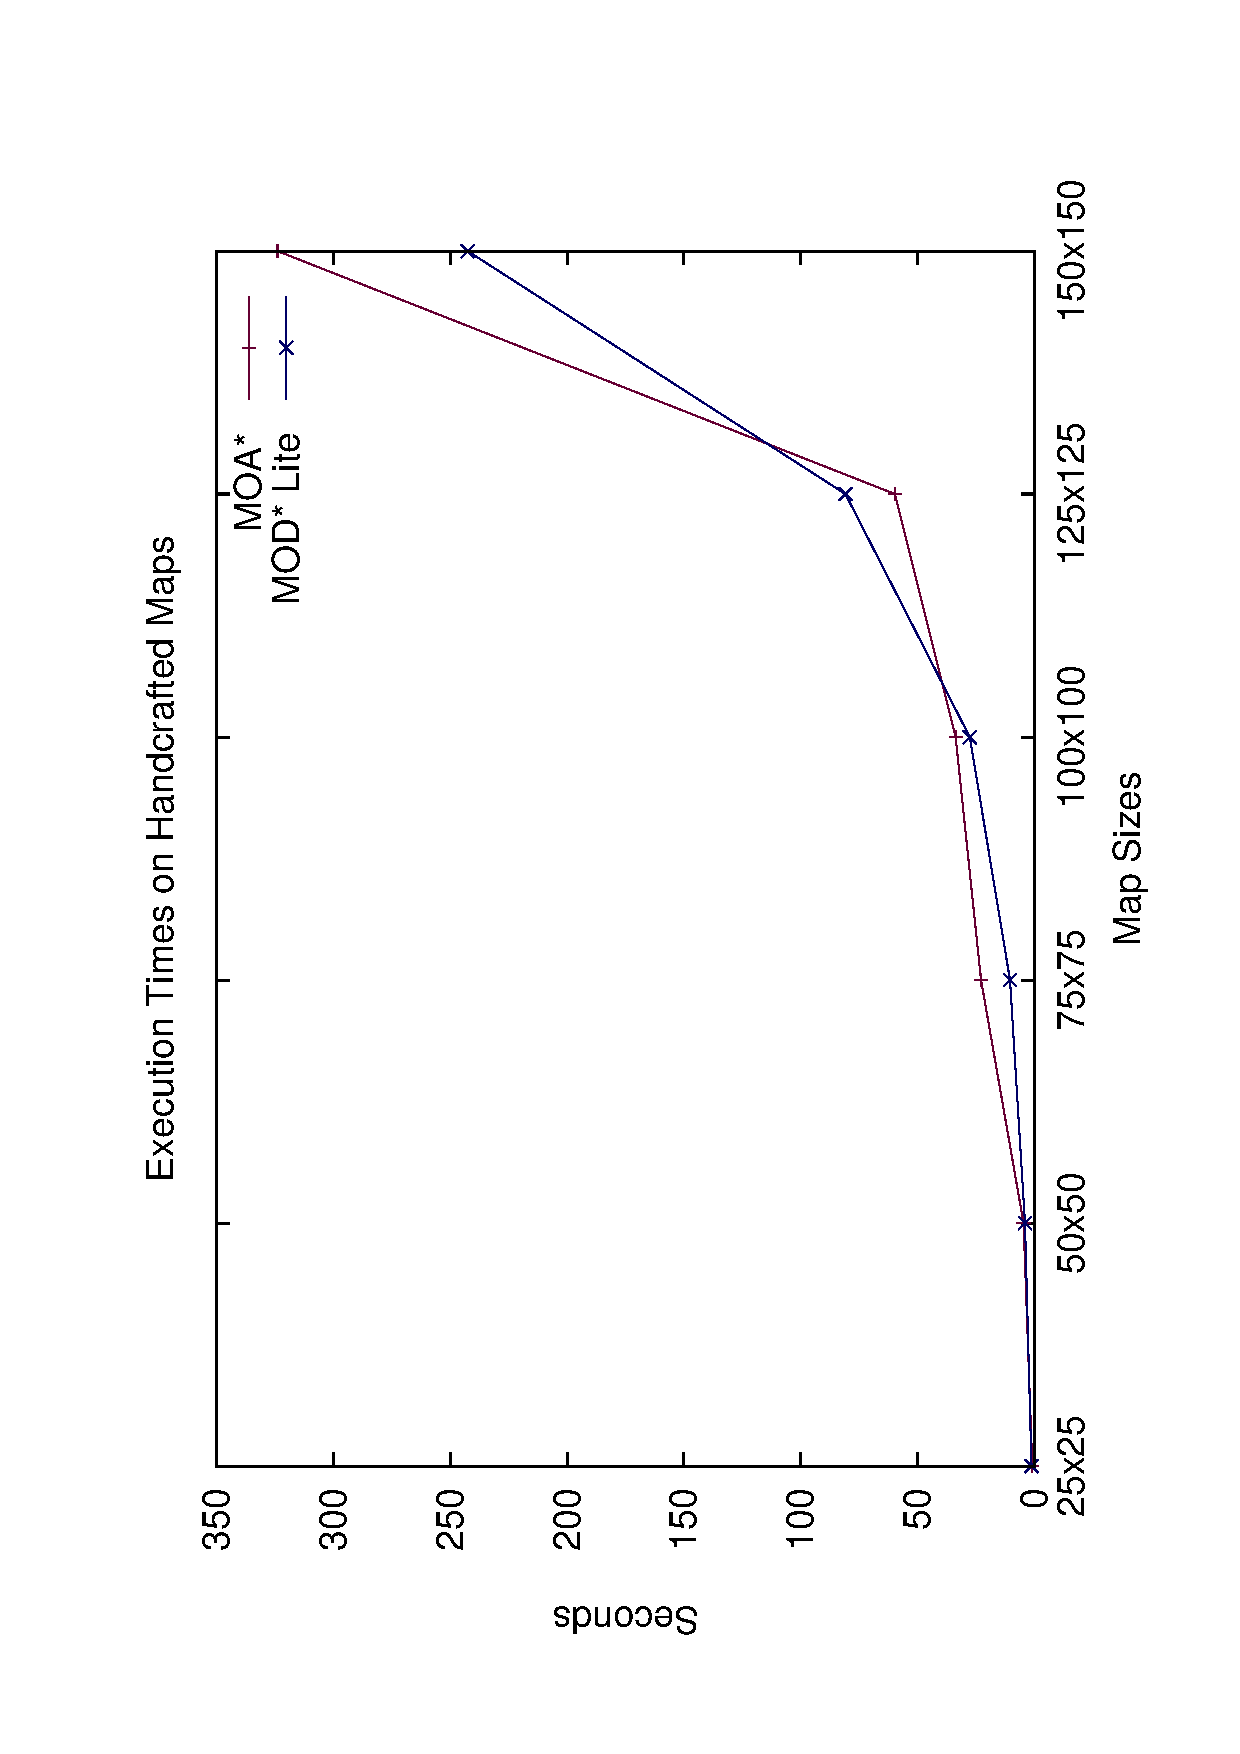
\includegraphics[scale=0.45]{experimental/handcrafted}
\caption{Execution Times of Handcrafted Fully Observable Maps}
\label{fig:hand_fully}
\end{figure}

\begin{table}[ht]
	\caption{Non-dominated Path Costs For Handcrafted Maps}
	\centering
    \begin{tabular}{l l l l l}
        \hline
        Map Size  &  MOD* Lite  & 	 MOA*  		&  	MOGPP		&	SPEA2\\ [0.5ex] \hline
        20 x 20   &	(39,264)	&	(39,264)	&	(39,1614)	&	(40,1273)
		   \cr    &	(41,258)	&	(43,6)		&	(41,394)	&	(44, 921)
   		   \cr    &	(45,0)		&	(45,0)		&	(47,264)	&	(46, 523)
   		   \cr	  &				&				&	(49,0)		&	(50, 176)
   		   \cr	  &				&				&				&	(74, 24)\\   		   
   		   \\
        40 x 40   & (79,528)	&	(79,528)	&	(95,1637)	&	(100, 3070)
		   \cr	  &	(81,352)	&	(81,352)	&	(115,880)	&	(106, 2648)
		   \cr	  &	(91,156)	&	(91,156)	&				&	(110, 2065)
		   \cr	  &	(97,0)		&	(97,0)		& 				&	\\
		   \\
        60 x 60   & (119,243)	&	(119,243)	&	(159,4761)	&	(162, 3525)
		   \cr	  & (123,33)	&	(123,33)	&	(165,1979)	&	(164, 211)
   		   \cr	  & (127,0)		&	(127,0)		&	(167,165)	&	
   		   \cr	  &				&				&	(233,99)	&	\\ 
   		   \\
        80 x 80   & (159,129)	&	(159,129)	&	(223,2327)	&	(222, 8122)
		   \cr	  &	(161,69)	&	(161,69)	&	(291,1627)	&	(236, 7833)
		   \cr	  &	(163,0)		&	(163,0)		& 				&	(258, 6314)
   		   \cr	  &				&				&				&	(292, 4565)
   		   \cr	  &				&				&				&	(322, 505)\\   		   
		   \\
        100 x 100 &	(199,30)	&	(199,30)	&	(311,4827)	&	(308, 6792)
		   \cr	  &	(201,6)		&	(201,6)		&	(327,3042)	&	(328, 4605)
		   \cr	  &	(203,0)		&	(203,0)		&	(341,1989)	&	(404, 2702)
   		   \cr	  &				&				&	(353,45)	&
   		   \cr	  &				&				&	(365,0)		&	\\ 
   		   \\
        120 x 120 & (239,77)	&	(239,77)	&	(363,11340)	&	(380, 30668)
		   \cr	  & (241,44)	&	(241,44)	&	(413,8821)	&	(390, 13316)
		   \cr	  &			   	&	(261,0)		&	(417,4613)	&	(400, 8362)   
		   \cr	  &			   	&				&	(455,3830)	&	(422, 8139)
		   \cr	  &			   	&				&	(517,1292)	&	(452, 4528)\\
		   \\
        140 x 140 & (210,1774)	&	(210,1774)	&	(306,16134)	&	(365, 10537)
           \cr	  & (212,1728)	&	(212,1344)	&	(336,10836)	&	
   		   \cr	  & (214,40)	&	(214,40)	&	(368,6510)	&	
		   \cr	  &	(244,0)	   	&	(244,0)		&	(390,4876)	&	
		   \cr	  &			   	&				&	(500,3335)	&	
		   \cr	  &			   	&				&	(514,2328)	&	\\
		   \\
        160 x 160 & (319,913)	&	(319,601)	&	(497,41016)	&	(544, 31061)
           \cr	  & (321,581)	&	(321,354)	&	(563,19675)	&	(634, 22045)
   		   \cr	  & (323,0)		&	(323,0)		&	(719,14811)	&	(776, 22022)
		   \cr	  &			   	&				&	(859,9448)	&	(840, 19231)\\ [1ex]
        \hline
    \end{tabular}
	\label{table:handPaths}
\end{table}

In Figure \ref{fig:hand_fully}, it can be seen that MOGPP increases gradually instead of an exponential growth especially on large scaled maps. However, its path quality is not good enough when compared to MOD* Lite and MOA*' s results.

MOD* Lite is much faster than MOA* and they both produce nearly similar results in path quality. This case shows that even MOD* Lite is developed for partially observable dynamic environments, it could also give \textit{as good results as} MOA* on stationary and fully observable environments and can be used for off-line use. For different path qualities of MOA* and MOD* Lite, we can say that the algorithm which find dominatable result finds the sub-optimal one instead of optimal.

\subsection{Partially Observable Tests}

As discussed in previous sections; the main difference of MOD* Lite from existing classic path planning or evolutionary based algorithms is its adaptivity to partially observable dynamic environments. To show this advantage, new tests are done with randomized maps of sizes 60 x 60, 80 x 80, 100 x 100 and 120 x 120. On these maps, agent's initial and target locations are again $(1, 1)$ and $(m, m)$ . For each map, agent' s sensor range was set between 10\% to 60\% and execution times were observed.

Example of the search space of MOD* Lite with 30\% sensor range is given in Figure \ref{fig:initialSearch}. In this figure, starting point is $(0,0)$ with green dot and target point is $(100,100)$ with red dot. Several threat zones are displayed all over the environment with pink dots. The more darkness a threat zone cell is, the more risk is exposured by agent. Inner cells of threat zones are designed to expose more risk. The fogged gray area represents agent' s sensor range on that particular iteration. The blue dot on $(40,47)$ is temporary goal, which must be the closest available cell to actual target within sensor range in regards of Manhattan distance. So on each iteration, temporary goal is re-calculated and paths are planned to that particular cell. Also calculated path can be seen as purple dots, from agent's current location -cyan dot- to temporary goal.

\begin{figure}
\centering
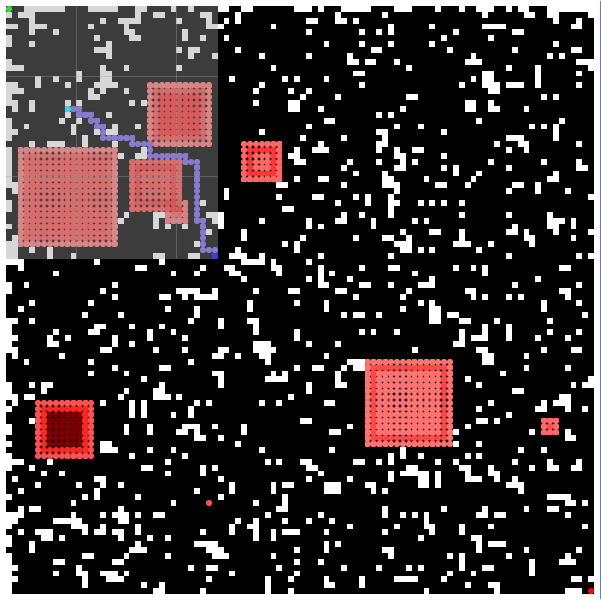
\includegraphics[scale=0.3]{experimental/initialSearch}
\caption{A 100x100 Partially Observable Map with 30\% Sensor Range}
\label{fig:initialSearch}
\end{figure}

In these tests, the agent starts to plan a path towards the nearest available cell within its sensor range -the temporary goal- to the actual goal with respect to Manhattan Distance. After planning, consider that agent has found three paths with costs $(15, 260)$, $(18, 230)$ and $(23, 200)$. In such cases, the agent tends to choose the path with cost $(18, 230)$, the median of paths. This ad-hoc strategy could be reconsidered according to the application domain. Afterwards, it starts to follow the chosen path. When new cells are available or a weight of a cell is changed within sensor range, agent reassigns the temporary goal and re-executes the path planner algorithm. This process iterates until the agent reaches to the desired goal location.

\begin{figure}
\centering
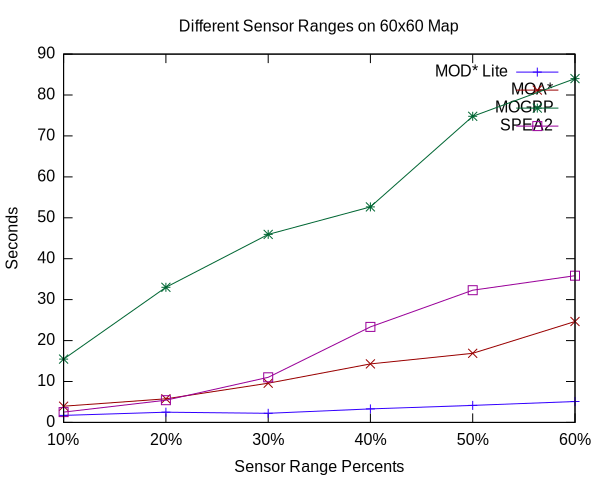
\includegraphics[scale=0.45]{experimental/60x60_partially}
\caption{60x60 Partially Observable Map on Different Sensor Ranges}
\label{fig:60x60sensor}
\end{figure}

\begin{figure}
\centering
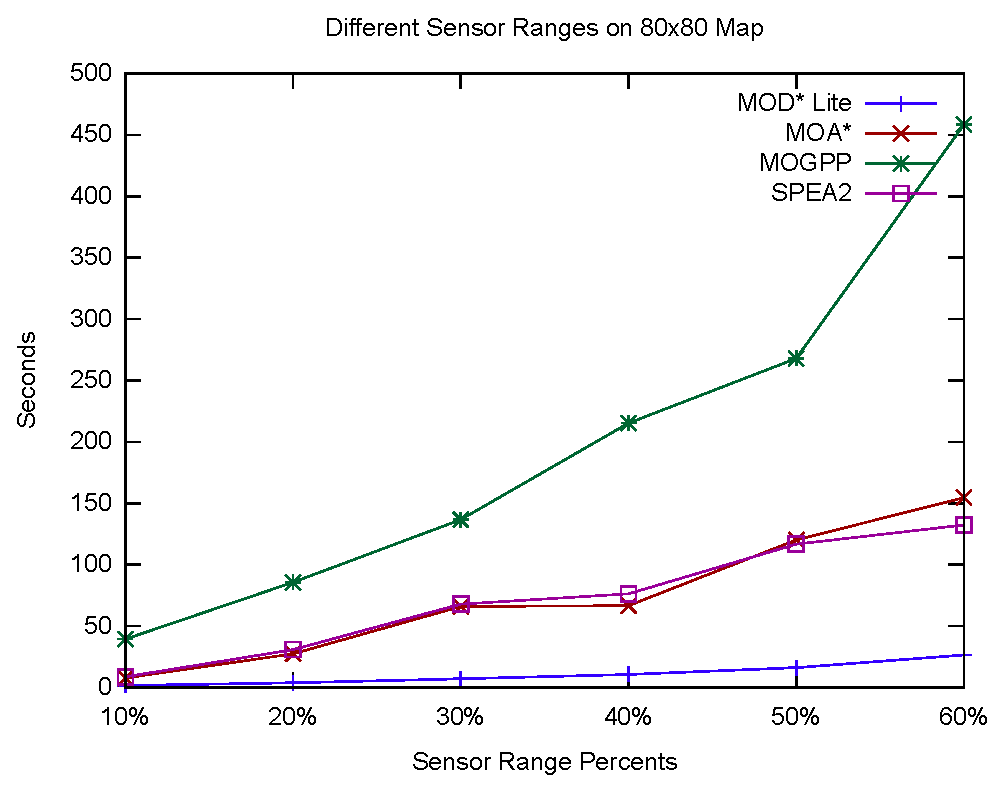
\includegraphics[scale=0.45]{experimental/80x80_partially}
%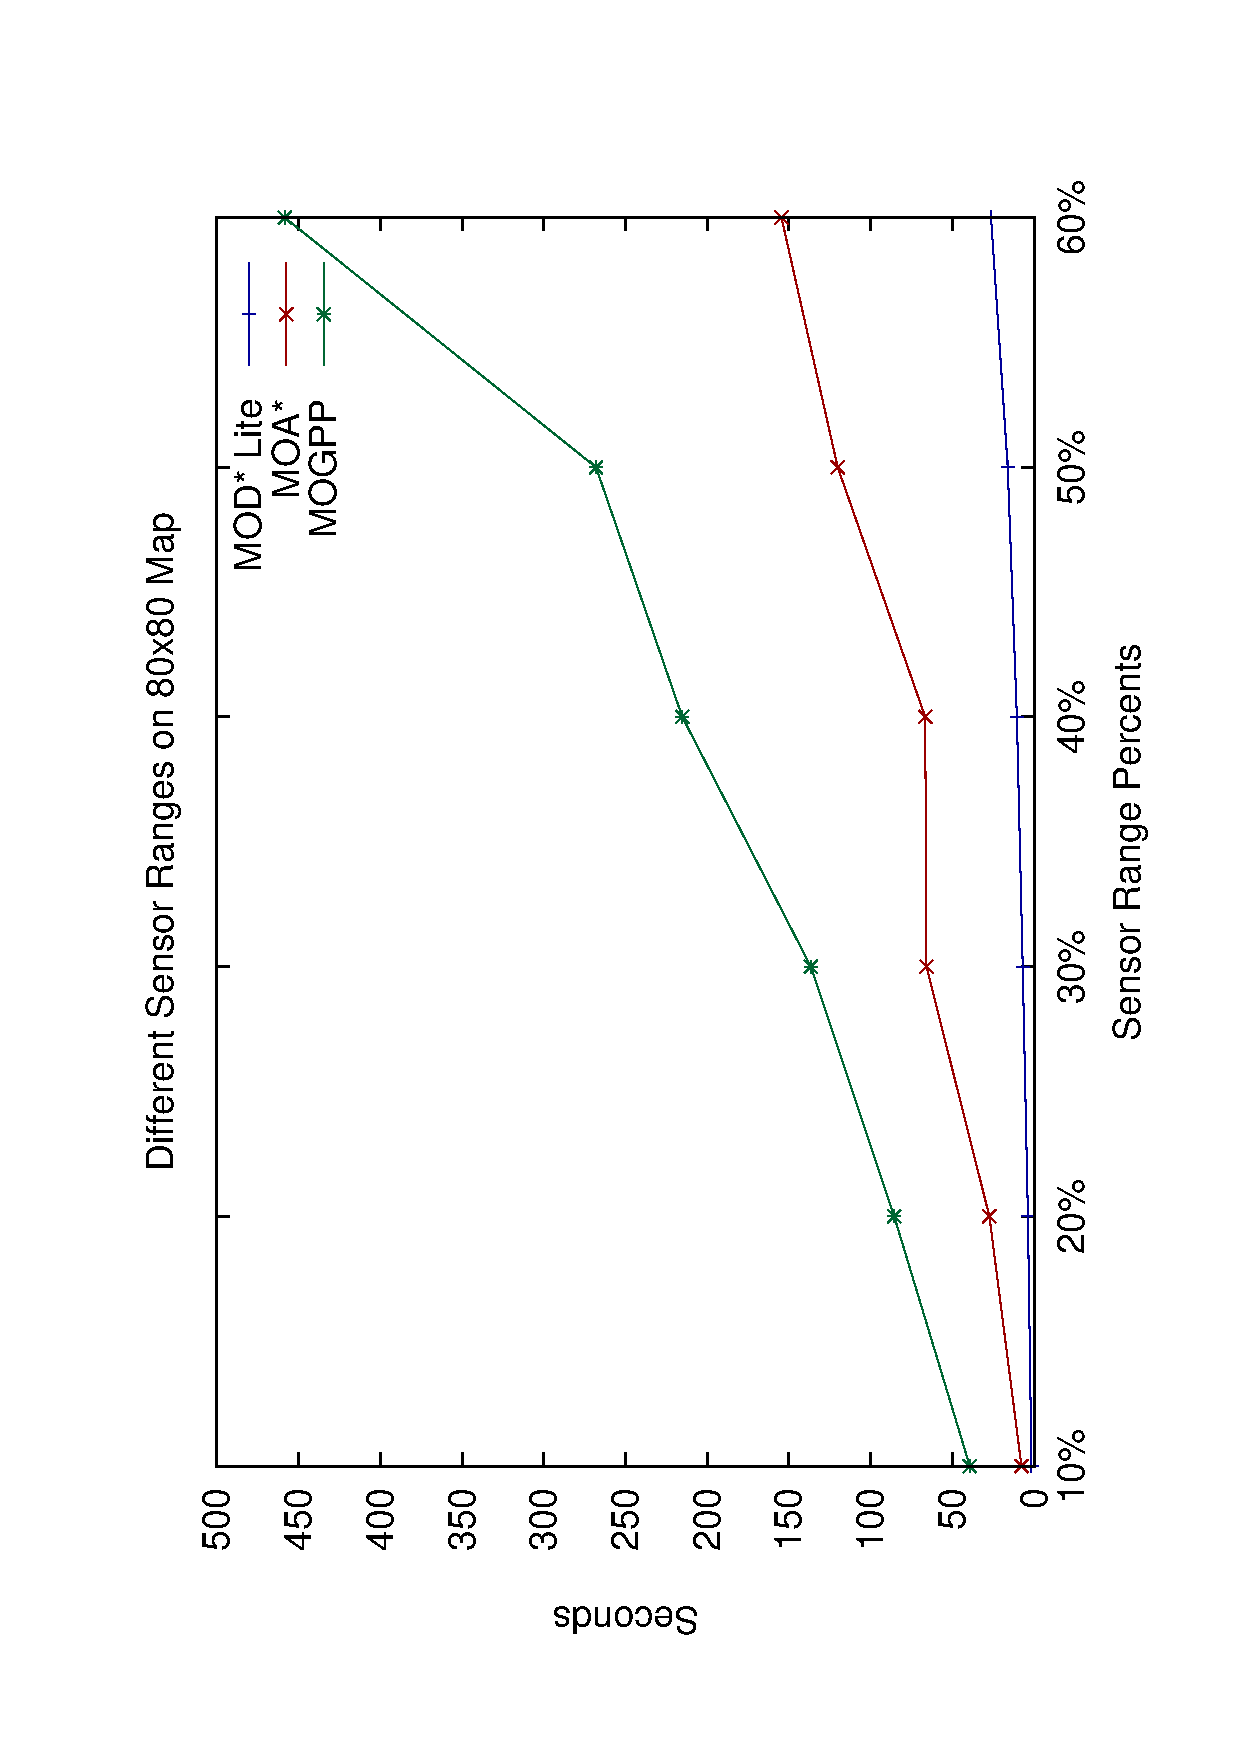
\includegraphics[width=2.0in,angle=270]{experimental/80x80_partially_normal}
\caption{80x80 Partially Observable Map on Different Sensor Ranges}
\label{fig:80x80sensor}
\end{figure}

\begin{figure}
\centering
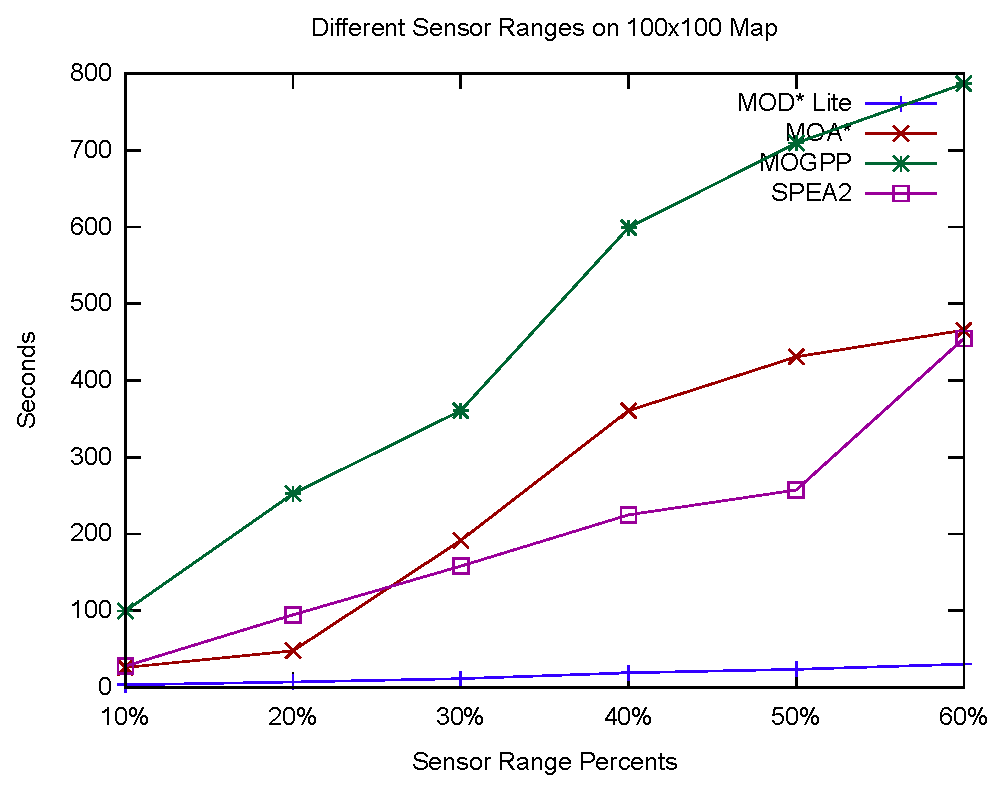
\includegraphics[scale=0.45]{experimental/100x100_partially}
\caption{100x100 Partially Observable Map on Different Sensor Ranges}
\label{fig:100x100sensor}
\end{figure}

\begin{figure}
\centering
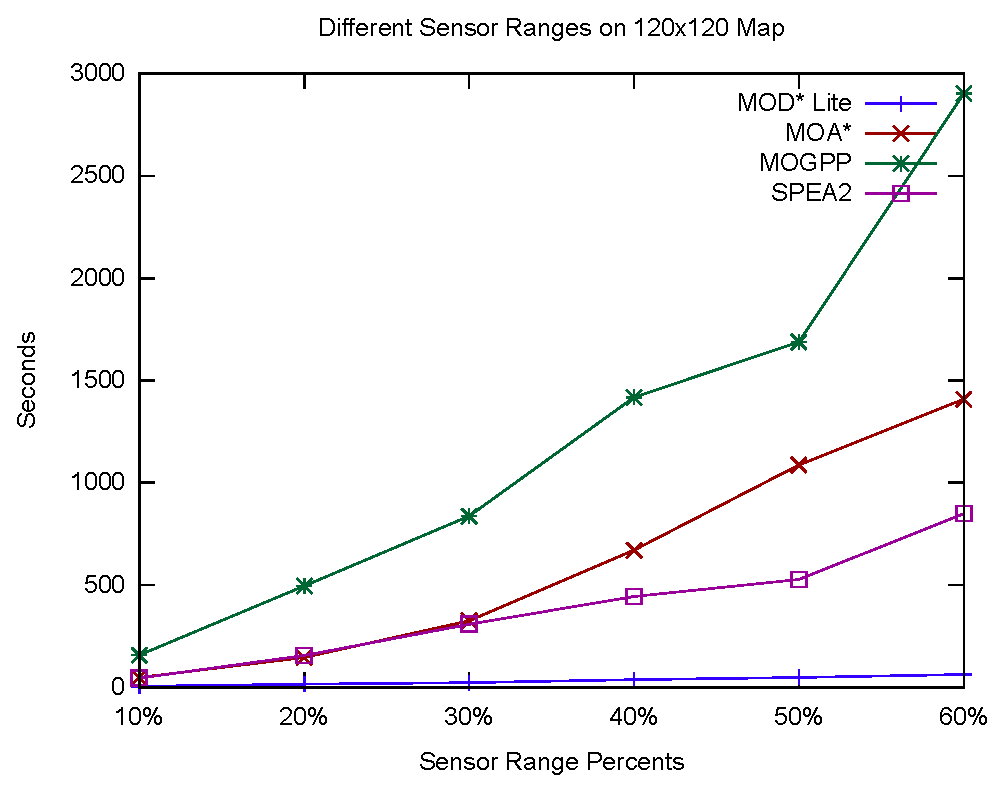
\includegraphics[scale=0.45]{experimental/120x120_partially}
\caption{120x120 Partially Observable Map on Different Sensor Ranges}
\label{fig:120x120sensor}
\end{figure}

%\begin{figure}
%\centering
%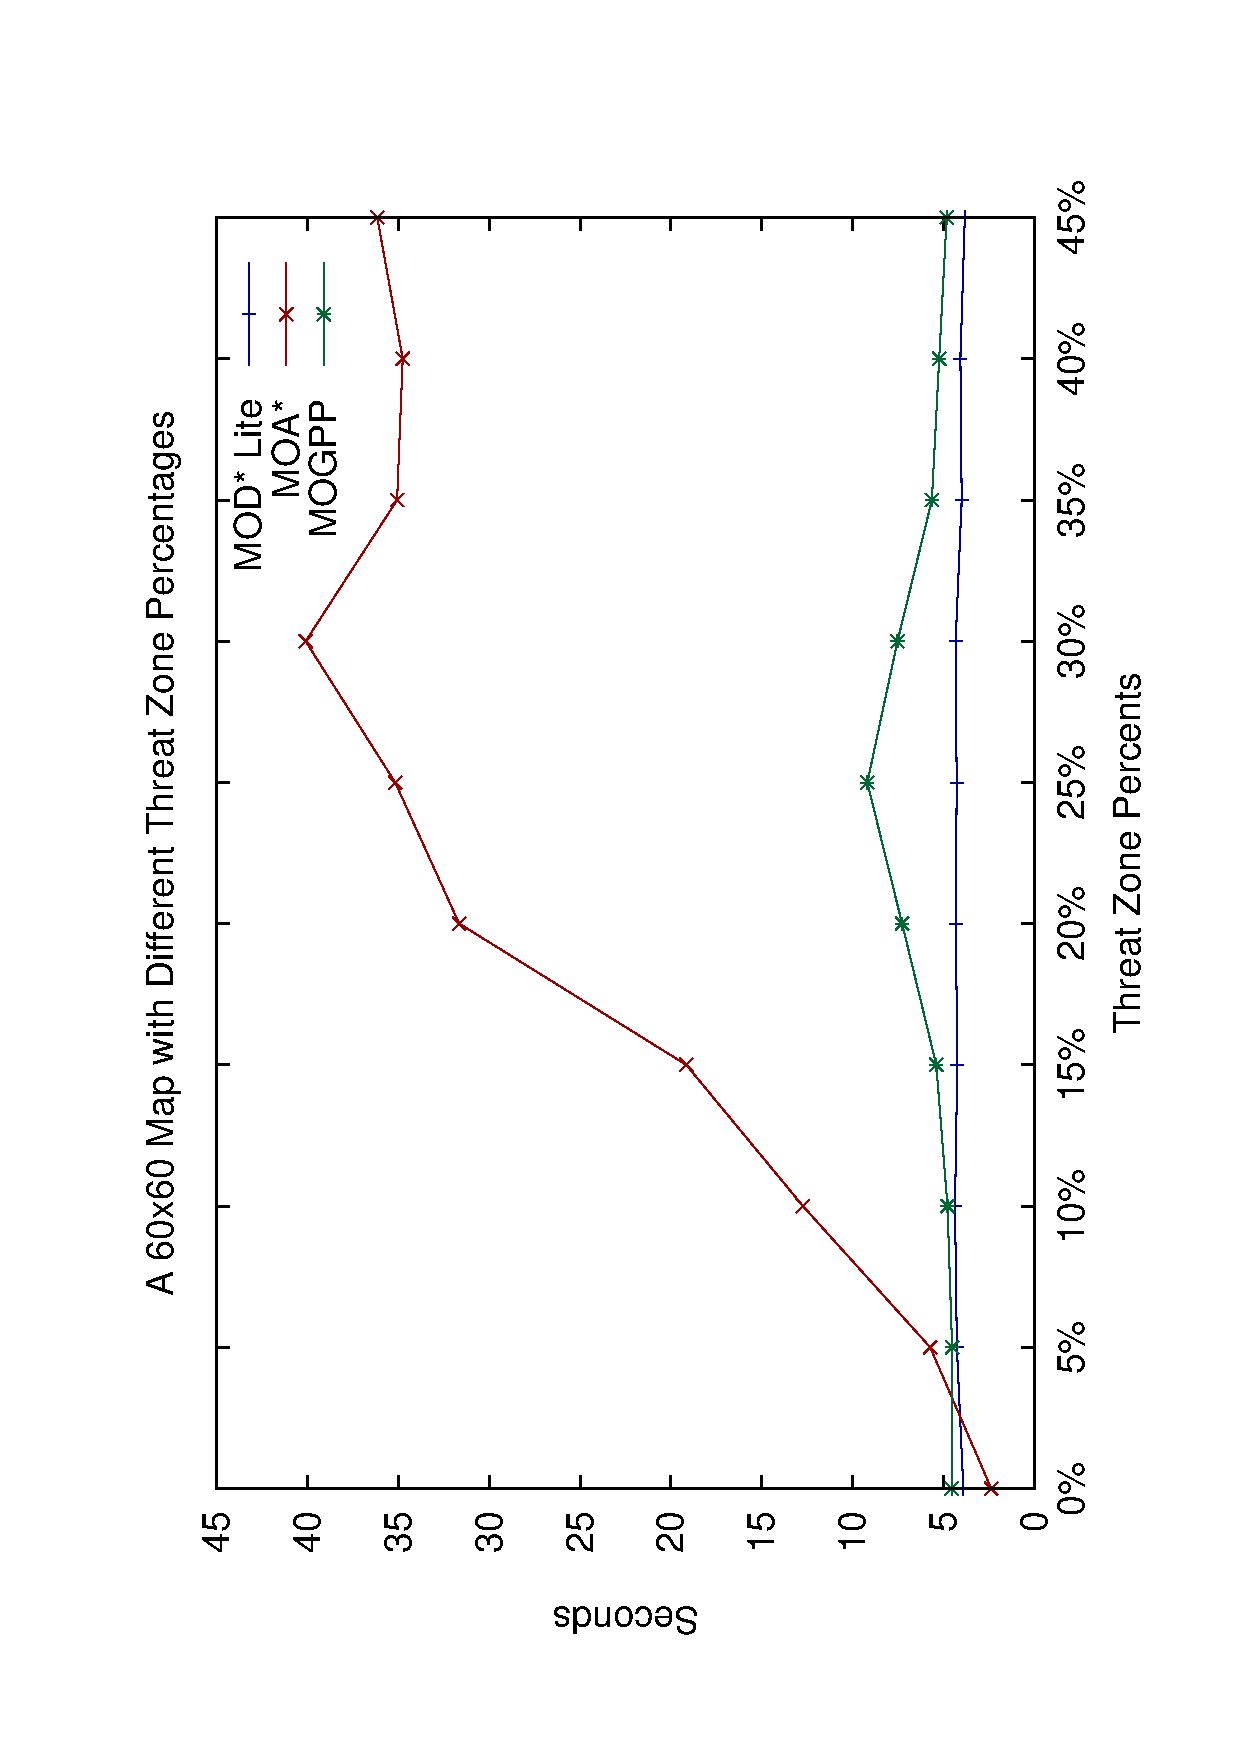
\includegraphics[width=2.5in]{experimental/60x60_multiobj_normal}
%\caption{Execution times of 60x60 Fully Observable Map on Different Threat Zone Percents}
%\label{fig:tzratio60}
%\end{figure}
%
%\begin{figure}
%\centering
%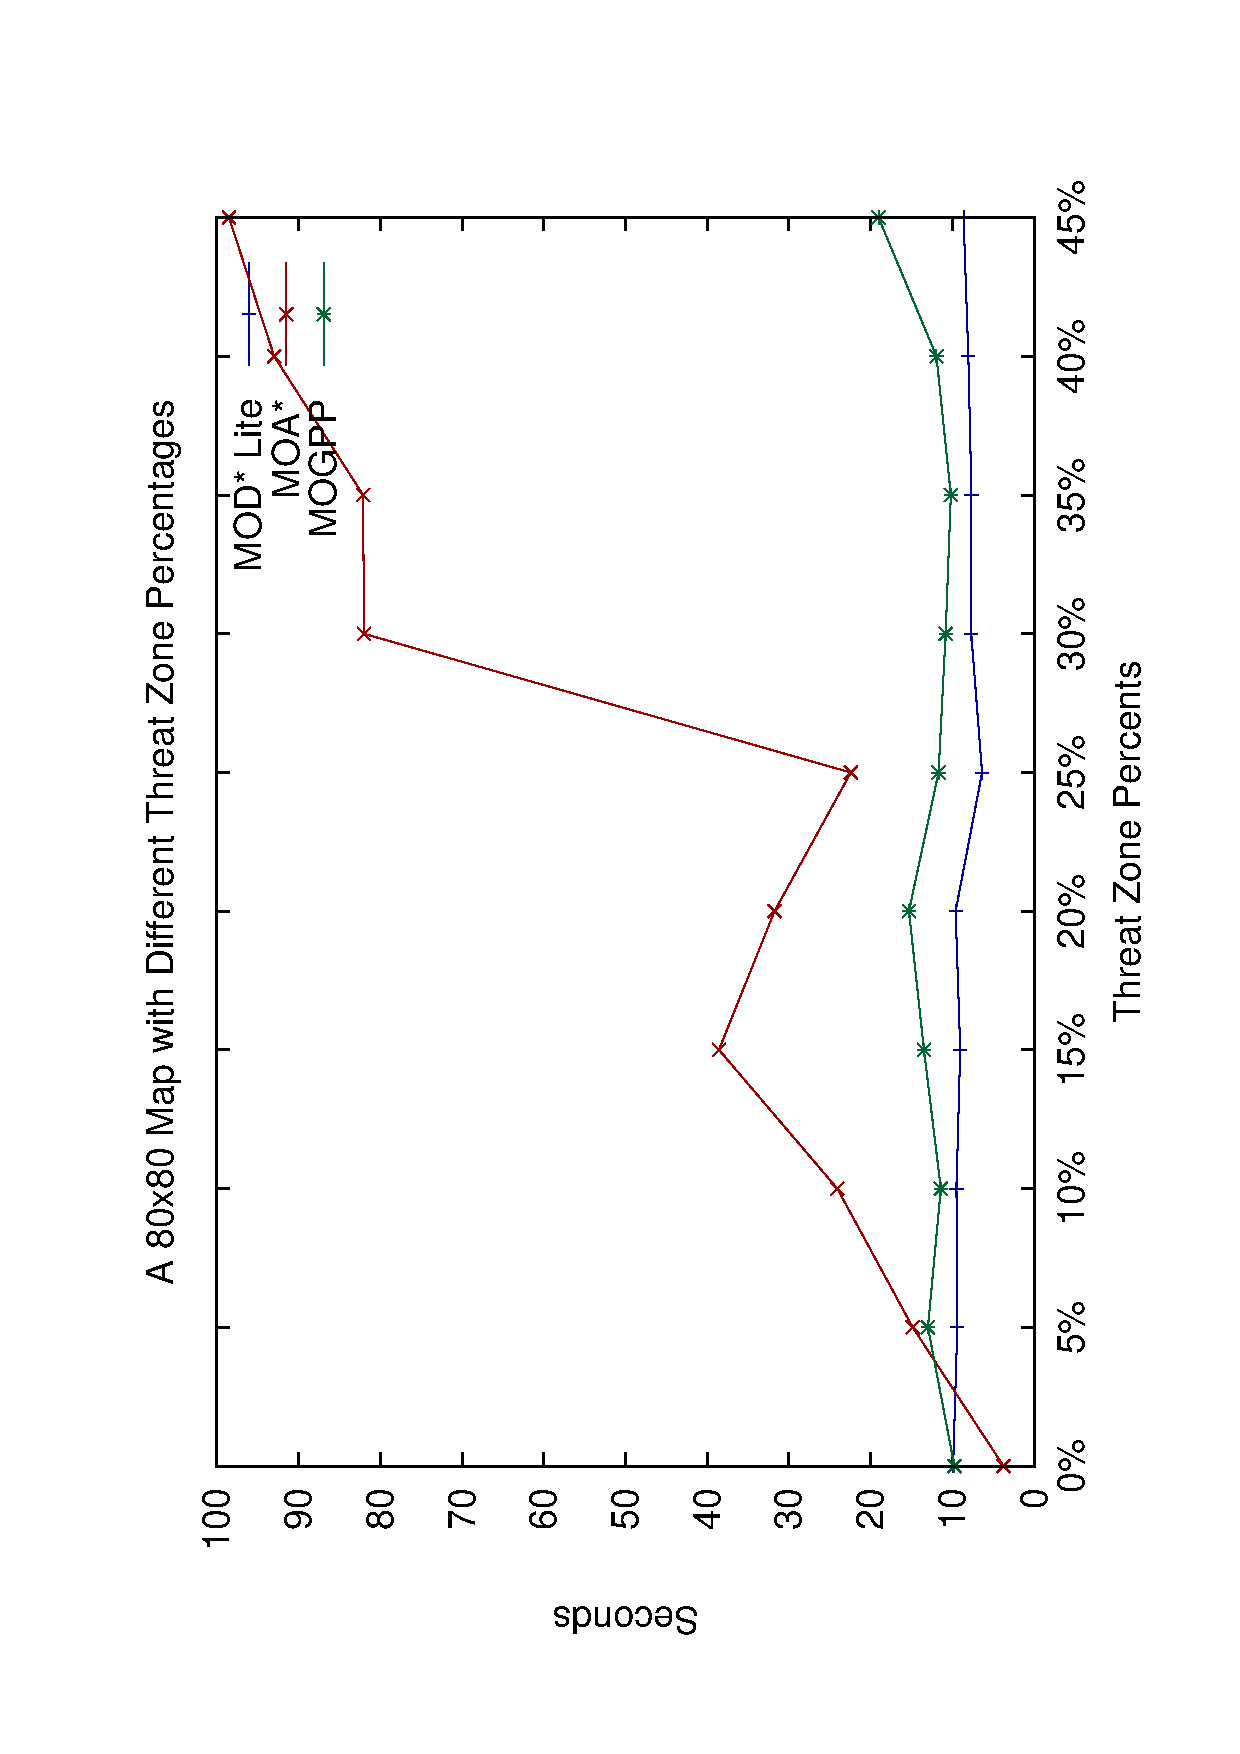
\includegraphics[width=2.5in]{experimental/80x80_multiobj_normal}
%\caption{Execution times of 80x80 Fully Observable Map on Different Threat Zone Percents}
%\label{fig:tzratio80}
%\end{figure}

%\begin{table}[ht]
%	\caption{MOGPP Execution Times on a 125x125 Partially Observable Map}
%	\centering
%    \begin{tabular}{l l}
%        \hline
%        Sensor Range	&	Execution Time (sec.)\\ [0.5ex] \hline
%        20\%			&	402.325\\
%        30\%			&	420.481\\
%		40\%			&	1024.237\\
%		50\%			&	1351.854\\
%		60\%			&	1922.415\\ [1ex]
%        \hline
%    \end{tabular}
%	\label{table:mogpp125vFrustum}
%\end{table}

\begin{table}[ht]
	\caption{Path Costs For Partially Observable Maps}
	\centering
    \begin{tabular}{l l l l l l}
        \hline
        Map Size	&	Sensor	&  MOD* Lite	& 	 MOA*	  	&  	MOGPP		&	SPEA2\\
					&	Range(\%)	&			&				&				&	\\ [0.5ex] \hline
        60 x 60		&	10		&	(126,124)	&	(132,0)		&	(136,248)	&	(144,0)
		   \cr		&	20		&	(124,124)	&	(120,0)		&	(148,18)	&	(158,0)
   		   \cr    	&	30		&	(118,0)		&	(118,0)		&	(142,0)		&	(198,0)
   		   \cr    	&	40		&	(118,0)		&	(118,0)		&	(144,0)		&	(234,626)
   		   \cr    	&	50		&	(118,0)		&	(118,0)		&	(168,0)		&	(262,36)
   		   \cr	  	&	60		&	(118,0)		&	(118,0)		&	(178,0)		&	(220,0)\\ 
   		   \\
        80 x 80		&	10		&	(170,0)		&	(158,0)		&	(194,116)	&	(262,134)
		   \cr		&	20		&	(162,0)		&	(158,0)		&	(186,283)	&	(326,0)
   		   \cr    	&	30		&	(162,0)		&	(158,0)		&	(252,142)	&	(288,295)
   		   \cr    	&	40		&	(162,0)		&	(166,0)		&	(258,259)	&	(372,582)
   		   \cr    	&	50		&	(162,0)		&	(158,0)		&	(266,233)   &	(352,325)
   		   \cr	  	&	60		&	(162,0)		&	(158,0)		&	(240,115)	&	(470,681)\\
   		   \\
        100 x 100	&	10		&	(198,0)		&	(198,0)		&	(254,715)	&	(394,1220)
		   \cr		&	20		&	(198,0)		&	(208,0)		&	(286,896)	&	(486,1064)
   		   \cr    	&	30		&	(198,0)		&	(198,0)		&	(294,1305)	&	(462,2959)
   		   \cr    	&	40		&	(198,0)		&	(198,0)		&	(398,2295)	&	(492,25)
   		   \cr    	&	50		&	(198,0)		&	(198,0)		&	(326,467)   &	(552,0)
   		   \cr	  	&	60		&	(198,0)		&	(198,0)		&	(370,928)	&	(712,969)\\ 
   		   \\
        120 x 120	&	10		&	(238,0)		&	(238,0)		&	(324,2141)	&	(450,0)
		   \cr		&	20		&	(238,0)		&	(238,0)		&	(382,124)	&	(442,0)
   		   \cr    	&	30		&	(238,0)		&	(238,0)		&	(464,0)		&	(550,646)
   		   \cr    	&	40		&	(238,0)		&	(238,0)		&	(448,0)		&	(730,57)
   		   \cr    	&	50		&	(238,0)		&	(238,0)		&	(542,0)		&	(746, 5857)
   		   \cr	  	&	60		&	(238,0)		&	(238,0)		&	(482,62)	&	(848, 0)\\	[1ex]
        \hline
    \end{tabular}
	\label{table:partiallyObsPathLengths}
\end{table}

The fundamental advantage of MOD* Lite can be seen very clearly on these tests. Similar to D* Lite, MOD* Lite is an incremental algorithm but MOA* is an offline algorithm. While MOD* Lite has the capability of updating only the effected states due to its incremental nature, MOA* re-plans the overall path from scratch when new parts become known and the weights of some cells have changed. This situation causes MOA*, MOGPP and SPEA2 to spend exponentially long times. Total execution times to reach to the target for all test cases are given in Figures \ref{fig:60x60sensor}, \ref{fig:80x80sensor}, \ref{fig:100x100sensor} and \ref{fig:120x120sensor}. Furthermore,  costs of the paths found by all algorithms are given in Table \ref{table:partiallyObsPathLengths}. As can be seen from results, MOD* Lite can easily handle ambiguities due to partial observability where all other three algorithms fail.  From these tests, it can be easily seen that MOD* Lite is extremely fast and it returns optimal or very near optimal solutions. However, MOA*, MOGPP and SPEA2 require exponential time and cannot be practically used. Notice that in a partially observable environment, as explorer agents are probable to discover different parts of the environment for different algorithms, paths with different path qualities might be yielded.

%As threat zones and their risk values are used as the second objective, percentages of these zones also affect execution time and generated path quality. In this set of tests different threat zone percents are tested on a fully observable 60 x 60 and 80 x 80 maps and results are given in Figure \ref{fig:tzratio60} and \ref{fig:tzratio80}, respectively. It could be observed that increasing risks of threat zones does not affect performances of  MOD* Lite and MOGPP too much, they find results in approximately similar times. However, MOA* is tightly coupled with it and execution time increases gradually as the threat percentage increases.

\section{Conclusion and Future Work}
\label{chapter:conclusion}

%Searching, path planning and navigation in real/virtual environments are vital issues and referred by many real-world applications in robotics. computer games, virtual simulations, etc.  Many solutions were introduced considering only a single optimization criteria; i.e., shortest path from an initial location to a target location. However, many real life problems require more complex situations with multiple objectives to be optimized. Furthermore, one should not ignore inaccessibility and dynamics of the real world and consider them for more realistic modeling. In a nutshell, a multi-objective search algorithm which can work on partially observable dynamic environments is required to satisfy all of these requirements.

In this paper, we propose a new method, MOD* Lite, for searching, planning and finding paths on known or unknown partially observable dynamic environments  where the agent needs to optimize more than one criteria that cannot be transformed to each other.  MOD* Lite is based on D* Lite and it brings multi-objectivity to the solution space successfully, which is required in many real-world problems. It is a domain independent algorithm and could be applied to any partially/fully observable dynamic environment with $n \ge 1$ different non-interacting objectives. It is compared with known and complete multi-objective off-line path planning algorithm, MOA*, well-known multi-objective evolutionary algorithm SPEA2 and with a novel evolutionary solution, multi-objective genetic path planner, MOGPP, based on solution quality and execution times. Experimental results show that MOD* Lite is able to optimize path quality and is fast enough to be used in real-world complex applications. To our best knowledge, MOD* Lite is the only incremental search method that can be used for optimizing multiple objectives in dynamic and partially observable search domains, which is classified as the hardest class of problems in state space search.

There exists several incremental {\it moving target} search algorithms in recent years \cite{Sun:2009}, \cite{GFR-A*Sun:2010}, \cite{MT-D*Lite:2010}. As a future research, we will attempt to extend our work for non-stationary targets. Also MOD* Lite could be reconsidered in multi agent environments where each agent autonomously executes its planner and cooperate with others to reach a target location. 

\bibliography{journal}{}
\bibliographystyle{ieeetr}

\end{document}
